% Set parameters
% set font size
\documentclass[11pt]{article}

% set line height
\renewcommand{\baselinestretch}{2}

% line number
\usepackage{lineno}

% today
\renewcommand{\today}{}

% set margin
\usepackage{geometry}
\geometry{a4paper, left=15mm, right=15mm, top=20mm, bottom=20mm}

% for using Korean
\usepackage{kotex}

% for using multi-languages
\usepackage[english]{babel}

% for urls
\usepackage{hyperref}

% for equation
\usepackage{amsmath}
\usepackage{mathtools}

% for fixing figure position
\usepackage{float}

% for citation
\usepackage{natbib}
\bibliographystyle{apa}
\setcitestyle{authoryear,open={(},close={)},citesep={;}}

% for drawing table
\usepackage{array,multirow,graphicx,rotating,booktabs}
\usepackage[table,xcdraw]{xcolor}

% for tabularx
\usepackage{tabularx}
\newcolumntype{b}{X}
\newcolumntype{s}{>{\hsize=.5\hsize}X}
\renewcommand\arraystretch{0.8} \setlength\minrowclearance{0.8pt}

% for itemize
\usepackage{enumitem}

%%%%%%%%%%%%%%%%%%%%%%%%%%%%%%%%%%%%%%%%%%%%%%%%%%%%%%%%%%%%%%%%%%%%%%%%%%%%%%%
\begin{document}

\title{Unsupervised Korean Natural Language Processing to Solve Out-of-Vocabulary and Dearth of Data}
\author{Hyunjoong Kim}

\maketitle
\smallskip

%%%%%%%%%%%%%%%%%%%%%%%%%%%%%%%%%%%%%%%%%%%%%%%%%%%%%%%%%%%%%%%%%%%%%%%%%%%%%%%
\section{Introduction}

자연어처리 (natural language processing) 는 사람의 언어를 컴퓨터가 이용할 수 있는 형태의 정보로 변환하고, 이를 이용하여 과업들 (tasks) 을 수행하는 분야이다.
자연어처리에서 수행하는 과업은 다양하다.
품사 판별과 형태소 분석은 텍스트를 단어열로 분해하는 전처리 과업에 해당한다.
단어의 특정 품사나 의미를 이해하는 객체명 인식과, 키워드나 핵심 문장을 이용하여 문서 집합을 요약하는 정보 추출 과업도 자연어처리에 포함된다.
또한 사용자의 질문에 대해 적절한 답변을 탐색하는 질의 응답도 자연어처리 과업에 포함된다.

자연어처리 과업의 많은 부분은 머신러닝 기법을 이용한다.
머신러닝은 학습 방식에 따라 세 가지로 분류할 수 있다.
지도기반 (supervised) 머신러닝은 객체의 특징을 기술하는 입력값 (input) 과 객체의 정답인 출력값 (output) 이 쌍으로 존재할 때 이를 이용하는 방식이다.
머신러닝 모델은 입력값으로부터 출력값을 예측하기에 유용한 정보를 학습한다.
품사 판별의 경우, 단어 - 품사 쌍으로 이뤄진 학습 데이터를 이용하여, 단어열이 입력되었을 때 이에 해당하는 품사열을 판별하는 정보를 모델이 학습한다.
이후, 새로운 단어열이 입력되면 적절한 품사열을 출력한다.
비지도기반 (unsupervised) 머신러닝은 데이터에 입력값만 존재할 때 쓰는 방법으로, 품사 판별의 경우, 두 단어가 앞 뒤에 등장하는 단어들의 분포가 비슷하면 하나의 품사로 이를 인식하는 Brown clustering \citep{brown1992class} 방법이 이에 해당한다.
강화학습 (reinforcement learning) 은 각 입력값에 대한 출력값은 주어지지 않았지만, 출력값에 대한 리워드 (reward) 를 정의할 수 있을 때 이용하는 방식이다.
출력값에 대하여 피드백을 줄 수 있는 도메인에서 이용할 수 있다.
대화 시스템에서 출력된 답변에 대한 피드백을 이용하여 답변 출력 방법을 수정하는 모델이 이에 해당한다 \citep{mo2018personalizing, singh2000reinforcement, li2016deep}. 

자연어처리의 많은 연구는 지도기반 머신러닝을 이용한다.
모델이 적용될 도메인의 입력값들을 포함하는 학습용 데이터를 구축한 뒤, 지도기반 모델을 이용하여 입력값과 출력값의 관계를 학습한다.
품사 판별의 경우, 단어 - 품사 쌍으로 이뤄진 말뭉치를 이용하여 한 단어의 앞, 뒤에 등장하는 문맥들을 고려하여 해당 단어의 품사를 추정하는 패턴을 학습한다.
품사 판별과 같은 과업은 텍스트 데이터를 벡터로 변환하는 전처리 과정에 이용되는 경우가 많기 때문에 결과값에 대한 피드백을 정의하기가 어렵기 때문에 지도기반 머신러닝 방법이 적합하다.

그러나 지도기반 머신러닝 방법을 이용하는 자연어처리 모델들은 공통적으로 다음과 같은 어려움이 있다.

\begin{enumerate}[noitemsep]
    \item \textbf{Out of vocabulary problem} : 학습 데이터에 등장하지 않은 단어를 제대로 인식하지 못하는 문제이다.
    \item \textbf{Dearth of Data} : 과업에 적합한 학습 데이터를 마련하기 어렵다.
    \item \textbf{Noise} : 텍스트 데이터에는 노이즈가 존재한다.
\end{enumerate}

첫째, 미등록 단어 문제는 학습 데이터를 이용하는 지도기반 머신러닝 방법에서는 필연적으로 발생하는 문제이다.
언어는 사용되는 시기와 도메인에 따라 다르기 때문에 한 종류의 학습 데이터에 모든 종류의 단어가 등장하지 않는다.
특히 품사 판별기와 같은 전처리 과업에서 자주 발생하는 문제로, 신조어와 같이 새롭게 만들어진 단어를 인식하지 못하여 문장이 잘못된 단어열로 분해된다.
이 결과를 이용하면 문장이나 문서를 잘못된 벡터로 표현되기 때문에 이후의 과업들의 성능이 저하된다.
라틴계 언어들은 단어를 띄어쓰기로 구분되며, 최근의 단어 임베딩 기법들을 이용하여 품사의 추정이 손쉽게 이뤄진다 \citep{turian2010word, mikolov2013efficient, collobert2011natural}.
하지만 단어의 경계가 띄어쓰기로 구분되지 않는 한국어, 중국어, 일본어에서는 미등록 단어를 제대로 인식하기 위해서는 추가적인 단어 사전 혹은 학습 데이터가 필요하다.

둘째, 학습 데이터가 존재하지 않거나, 이를 구축하기 어려운 경우들이 많다.
객체명 인식은 장소, 사람과 같이 단어의 의미적 클래스를 분류하는 과업이다.
지도학습 기반으로 객체명 인식 모델을 학습하려면 각 클래스가 태깅된 학습 데이터가 필요하다.
하지만 객체명 인식이 필요한 도메인마다 단어 클래스가 다르기 때문에 새롭게 학습 데이터를 구축해야 한다.
영화 제목을 인식하는 객체명 인식 모델을 학습하기 위해서는 영화 제목이 태깅된 학습 데이터가 필요하다.

셋째, 텍스트 데이터에는 노이즈가 존재한다.
특정 과업을 위해 태깅된 데이터를 구하기는 어렵지만, 레이블이 존재하지 않는 텍스트 데이터를 구하는 것은 어렵지 않다.
많은 양의 텍스트 데이터는 사람에 의하여 제작되기 떄문에 띄어쓰기 오류나 철자법 오류가 존재한다.
사전을 이용하는 품사 판별기는 철자법이 틀린 단어를 제대로 인식할 수 없다.
또한 띄어쓰기가 제대로 지켜지지 않으면 단어 간의 경계를 제대로 인식하지 못한다.
자연어처리 과업의 성능을 높이기 위해서는 노이즈를 제거하는 과정이 필요하다.

이 논문에서는 다음의 한국어 자연어처리 과업에서 발생하는 위의 세 가지 문제를 해결하는 방법들을 제안한다.

\begin{enumerate}[noitemsep]
    \item Korean space error correction
    \item Enhancing part of speech tagging with unsupervised word extraction
    \item Keyword extraction
\end{enumerate}

첫째, 한국어 문서의 띄어쓰기 오류를 교정한다.
한국어는 띄어쓰기 오류가 일부 포함되어도 가독이 어렵지 않기 때문에 띄어쓰기 오류가 자주 발생한다.
띄어쓰기 오류 교정은 글자 단위의 순차적 판별 (sequential labeling) 문제이기 때문에 순차적 판별 알고리즘들이 이용될 수 있다.
이들은 띄어쓰기 오류가 없는 학습 데이터로부터 글자열에 가장 적합한 띄어쓰기 품사열을 출력한다.
그러나 도메인마다 사용되는 어휘가 다르기 때문에 각 도메인에 적합한 학습 데이터를 마련해야 한다.
3 장에서 일부 띄어쓰기 오류가 포함된 학습 데이터로도 안정적인 띄어쓰기 교정을 하는 방법을 제안한다.
또한 학습 데이터의 띄어쓰기 오류 수준에 따른 교정 능력의 변화도 확인한다.

둘째, 단어 추출 기법을 이용하여 한국어 품사 판별의 성능을 높인다.
품사 판별은 미등록단어 문제를 자주 겪는다.
특히 단어의 경계가 명확히 기록되지 않는 한국어에서는 미등록단어가 작은 단위의 형태소들로 분해되는 문제가 자주 발생한다.
이를 방지하기 위하여 한국어 품사 판별기들은 사용자가 직접 사전을 추가하는 기능을 제공하지만, 사용자 사전의 구축은 사용자의 몫이다.
단어 추출 기법은 문서 집합에서 통계 기반으로 단어를 추출하는 방법이다.
4 장에서 단어 추출 기법을 품사 판별 과업 모델에 추가하여 각 도메인에 적합한 사용자 사전을 스스로 구축하는 품사 판별기를 제안한다.

셋째, 비지도학습 기반 키워드 추출 기법을 제안한다.
키워드 추출 기법은 문서 요약에 이용되는 대표적인 방법이다.
하지만 각 문서나 문서 집합에 적합한 키워드가 무엇인지 태깅된 학습 데이터는 잘 존재하지 않기 때문에 비지도학습 기반의 방법들이 제안되었다.
키워드 추출 기법은 데이터의 성질에 따라 다르게 접근해야 한다.
문서 집합이 동일한 주제에 대한 문서들로 구성되었을 경우 (homogeneous data), TextRank \citep{mihalcea2004textrank} 같은 그래프 랭킹 기반 알고리즘이 이용될 수 있다.
하지만 TextRank 는 단어열이 제대로 분해되었을 경우 잘 작동한다.
5.1 장에서 데이터기반으로 미등록단어 문제를 해결하며 키워드를 추출하는 한국어 텍스트를 위한 그래프 갱킹 기반 방법을 제안한다.
문서 집합이 서로 다른 주제의 문서들로 구성된 경우 (heterogeneous data), 그래프 랭킹 기반 알고리즘은 빈도수가 높은 일반적인 단어들을 키워드로 선택한다.
이를 해결하기 위해서 문서 집합을 주제별로 구분하여야 한다.
5.2 장에서 문서 군집화 기법을 이용하여 문서 집합을 분류한 뒤, 각 문서 군집을 구분할 수 있는 단어를 키워드로 선택하는 방법을 제안한다.

이 논문에서 제안하는 방법들은 순차적 판별 알고리즘, 단어 임베딩 기법, 그리고 키워드 추출 알고리즘이 이용된다.
2 장에서는 이에 대하여 살펴본다.

%%%%%%%%%%%%%%%%%%%%%%%%%%%%%%%%%%%%%%%%%%%%%%%%%%%%%%%%%%%%%%%%%%%%%%%%%%%%%%%
\section{Related work}

\subsection{Structure of Korean}

한국어의 문장은 어절로 구성되어 있으며, 어절은 띄어쓰기를 기준으로 나뉘는 단위이다.
한 어절은 하나의 단어 혹은 여러 개의 단어로 구성될 수 있다.
그리고 단어는 하나 이상의 형태소로 구성된다.
한국어의 단어 품사는 5언 9품사이며, 각 단어는 그 자체로 형태소 품사를 지닌다.
단 형용사와 동사는 용언의 어간과 어미 형태소로 구성된다.

"이것은 예문 입니다" 라는 문장은 세 개의 어절로 구성되어 있으며, "이것은" 어절은 "이것/명사 + 은/조사"로 구성된다.
"입니다"는 하나의 단어인 "입니다/형용사"로 구성되어 있는데, 이는 "이/형용사 어간 + ㅂ니다/어미"라는 두 개의 형태소로 구성된다.
"예문"은 하나의 형태소가 하나의 단어를 이루며, 하나의 단어가 하나의 어절을 이룬 경우이다.

\begin{figure}[H]
\centering
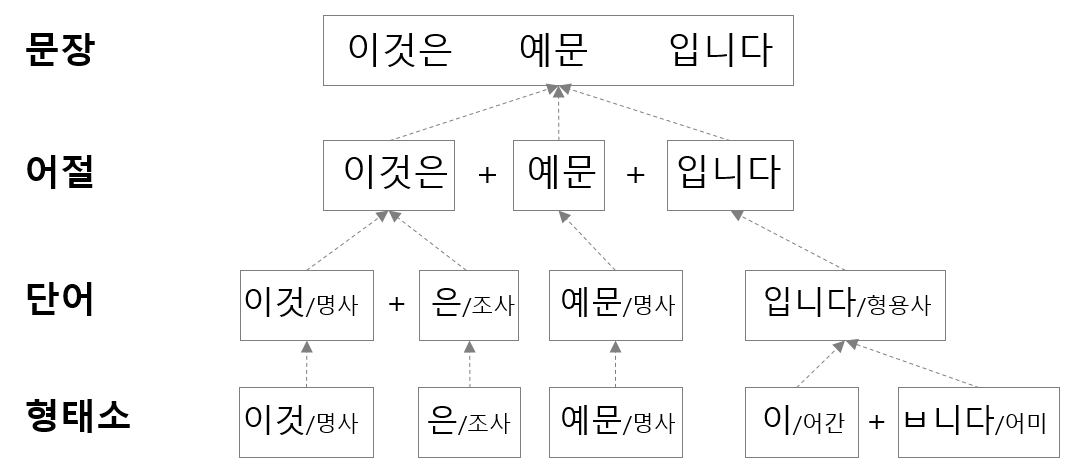
\includegraphics[keepaspectratio=true, width=0.8\linewidth]{figures/korean_structure.png}
\caption{한국어의 문장은 어절로, 어절은 단어로, 단어는 형태소로 구성되어 있다.}
\label{fig:korean_structure}
\end{figure}

%%%%%%%%%%%%%%%%%%%%%%%%%%%%%%%%%%%%%%%%%%%%
\subsection{Word embedding}

언어 모델 (language model) 은 문장의 생성 확률을 표현하기 위한 방법으로, 처음 제안되었을 때는 식 \ref{eq:slm} 처럼 n-gram 에 기반하여 문장의 확률을 정의하였다 \citep{jurafsky2014speech}.

\begin{equation}
  \label{eq:slm}
  \begin{aligned}
  P(w_{1:p}) = \prod_i P(w_i \vert w_{i-n+1:i-1}) \\
  P(w_i \vert w_{i-n+1:i-1}) = \frac{\#(w_{i-n+1:i})}{\#(w_{i-n+1:i-1)}}
  \end{aligned}
\end{equation}

그러나 이는 n-gram 종류 증가에 따른 모델의 크기 증가하는 문제와 단어 간 의미적 유사성을 표현하지 못하는 단점이 있었고, 이를 해결하기 위하여 피드 포워드 뉴럴 네트워크 기반 언어 모델이 제안되었다 \citep{bengio2003neural}.
\citep{bengio2003neural} 의 언어 모델은 각 단어를 고정된 크기의 임베딩 벡터로 표현한 뒤, $w_{i-n-1:i-1}$ 단어의 벡터를 연결한 입력값으로 $w_i$ 단어를 예측하는 2 층 피드 포워드 뉴럴 네트워크를 제안하였다 (식 \ref{eq:nlm}).

\begin{equation}
  \label{eq:nlm}
  \begin{aligned}
  y = b + Wx + U \cdot tanh(d + Hx) \\
  x = (C(w_{i-n+1}), \dots, C(w_{i-1})), y = w_i
  \end{aligned}
\end{equation}

그 결과 비슷한 문맥에서 등장하는 단어는 비슷한 임베딩 벡터로 표현되었다.
하지만 식 \ref{eq:nlm} 은 오랜 학습 시간이 필요하였다.
Mikolov 는 Word2Vec 이라는 뉴럴 네트워크의 입력값과 출력값의 벡터 크기를 동일하게 만들기 위하여 $n-1$ 개 단어의 벡터값의 평균을 입력값으로 변환하여 $w_i$ 를 예측하는 softmax regression 으로 모델을 간략히 만들었다 \citep{mikolov2013efficient}.
Bengio 의 모델은 한 단어의 앞에 등장한 단어만 입력값으로 이용하였는데, Mikolov 는 뒤에 등장한 문맥도 고려하기 위하여 한 단어의 앞, 뒤에 등장하는 $w$ 개의 단어의 임베딩 벡터의 평균을 입력값으로 이용한다 (식 \ref{eq:word2vec}).

\begin{equation}
  \label{eq:word2vec}
  \begin{aligned}
  P(w_i \vert w_c) = \frac{exp(w_i^T w_c)}{\sum_j exp(w_j^T w_c)} \\
  w_c = avg(w_{i-w}, \dots, w_{i-1}, w_{i+1}, \dots, w_{i+w})
  \end{aligned}
\end{equation}

또한 클래스의 개수가 단어 개수인 softmax regression 의 학습을 효율적으로 하기 위하여 Noise Contrastive Estimation \citep{gutmann2010noise} 에 기반한 negative sampling 기법을 적용하였다 \citep{mikolov2013distributed}.
그 결과 뉴럴 네트워크 기반 언어 모델처럼 단어의 의미적 정보가 보존된 임베딩 벡터를 빠른 시간 내에 학습할 수 있게 되었다.

GloVe 는 두 단어의 임베딩 벡터를 이용하여 두 단어가 $w$ 간격 안에 함께 등장할 빈도수 $X_{i,j}$ 를 직접 예측하는 regression 문제로 단어 임베딩 벡터를 학습한다 \citep{pennington2014glove}.
식 \ref{eq:glove} 처럼 두 단어 $i, j$ 의 임베딩 벡터 $w_i, w_j$ 의 내적에 bias $b_i, b_j$ 를 더한 값이 co-occurrence 의 로그값 $log(X_{i,j})$ 에 가까워지도록 $w, b$ 를 학습한다.
자주 등장한 단어에 대하여 임베딩 벡터가 더 잘 학습되도록 증가함수 $f(X_{i,j})$ 를 이용하여 각 단어의 손실양에 가중치를 더한다.

\begin{equation}
  \label{eq:glove}
  minimize \sum f(X_{i,j}) \cdot \left( w_i^t w_j + b_i + b_j - log(X_{i,j}) \right)^2
\end{equation}

Word2Vec 과 GloVe 는 Harris 의 "비슷한 의미를 지닌 단어는 비슷한 문맥에서 등장한다"는 가정을 기반으로 임베딩 벡터를 학습한다 \citep{harris1954distributional}.
Word2Vec 은 softmax regression 을 이용하여 비슷한 문맥 (비슷한 입력값)을 지니는 두 단어가 비슷한 임베딩 벡터가 되도록 학습한다.
GloVe 는 단어 $j$ 의 인덱스를 고정할 경우 단어 $i$ 에 대한 선형 회귀식이 되며, 비슷한 문맥에서 등장한 단어는 비슷한 회귀 계수를 지니게 된다.
그리고 Word2Vec 과 GloVe 는 비슷한 단어 임베딩 벡터를 학습한다고 알려졌다 \citep{levy2015improving}

또한 negative sampling 을 이용하는 Word2Vec 의 한 종류인 Skip-gram (SGNS) 은 단어 간 co-occurrence 행렬에 Shifted PMI 를 적용한 공간과 같음이 증명되었다 \citep{levy2014neural}.
식 \ref{eq:levy_pmisvd} 의 $\vec{c}, \vec{w}$ 는 SGNS 의 문맥 단어와 기준 단어의 임베딩 벡터이며, 이들의 내적은 두 단어의 co-occurrnce 의 PMI 값에서 negative samples 의 개수인 $k$ 의 로그값을 뺀 것과 동치임이 증명되었다.
한 단어는 문맥 단어와의 co-occurrence matrix 에 Shifted PMI 를 적용한 벡터로 표현할 수 있다 \citep{levy2014neural}.

\begin{equation}
  \label{eq:levy_pmisvd}
  \vec{w} \cdot \vec{c} = log \left( \frac{\#(w,c) \cdot \vert D \vert}{\#(w) \cdot \#(c)} \cdot \frac{1}{k} \right) = log \left( \frac{\#(w,c) \cdot \vert D \vert}{\#(w) \cdot \#(c)} \right) - log k
\end{equation}

Word2Vec 과 같은 distributed representation 으로 이를 표현하기 위해서 SVD 를 적용할 수 있는데, 식 \ref{eq:better_svd} 처럼 고유값 (eigen value) 행렬을 단어와 문맥 행렬에 나눠 곱해야 SGNS 과 비슷한 단어 임베딩 벡터 $W^{SVD}$ 를 얻을 수 있다 \citep{levy2015improving}.

\begin{equation}
  \label{eq:better_svd}
  \begin{aligned}
  M_d = U_d \cdot \Sigma_d \cdot V_d^T \\
  W^{SVD} = U_d \cdot \Sigma_d^{0.5} \\
  C^{SVD} = V_d \cdot Sigma_d^{0.5}
  \end{aligned}
\end{equation}


그러나 Word2Vec, GloVe, PMI+SVD 와 같은 단어 임베딩 방법은 빈도수가 작은 단어나 학습 데이터에 등장하지 않은 단어에 대해서는 단어 임베딩 벡터를 얻기가 어렵다.
FastText 는 빈도수가 적은 단어와 미등록단어의 임베딩 벡터를 표현하기 위하여 한 단어의 임베딩 벡터를 구성하는 서브워드의 임베딩 벡터의 합으로 표현한다 \citep{bojanowski2017enriching}.
예를 들어 'where' 라는 단어의 임베딩 벡터는 단어의 경계를 표현하기 위하여 단어에 (, ) 를 추가한 뒤, '(where)' 의 3 ~ 6 글자의 서브워드인 '(wh, whe, ..., where)' 의 임베딩 벡터의 합으로 표현한다.
이를 SGNS 의 단어 임베딩 벡터로 이용하여 학습한다.
그 결과 비슷한 문맥에서 이용되는 서브워드는 비슷한 임베딩 벡터로 표현되며, 형태가 비슷한 단어는 비슷한 서브워드들로 구성되기 때문에 비슷한 임베딩 벡터로 표현된다.

이러한 단어 임베딩 벡터는 이후 다른 자연어처리 과업의 pre-trained 된 벡터로 이용되며, 미등록단어 문제를 해결하기도 한다.
한 문서 집합의 모든 단어를 이용하여 임베딩 벡터를 학습한 뒤 품사 정보가 태깅된 일부 단어를 이용하여 뉴럴 네트워크 기반 품사 판별기를 학습하면 품사 정보가 없는 단어에 대해서 비슷한 임베딩 벡터를 지니는 단어로 품사 태깅이 가능하다.

또한 단어 임베딩 벡터는 각 과업에 따라 단어 벡터가 변할 수 있다.
앞의 단어 임베딩 방법을 이용하면 'good' 과 'bad' 는 비슷한 문맥에서 등장하기 때문에 비슷한 벡터로 학습되지만, 감성 분삭 과업에 의하여 fine-tune 을 하면 서로 다른 벡터로 변환된다 \citep{kim2014convolutional, joulin2016bag}.

%%%%%%%%%%%%%%%%%%%%%%%%%%%%%%%%%%%%%%%%%%%%
\subsection{Sequential labeling}

시퀀스 레이블링 기법은 길이가 $n$ 인 입력 시퀀스 $x = [x_1, x_2, \dots, x_n]$ 에 대하여 가장 적절한 출력 시퀀스 $y = [y_1, y_2, \dots, y_n]$ 을 출력하는 머신러닝 알고리즘이다 (식 \ref{eq:sequential_labeling}).

\begin{equation}
  \label{eq:sequential_labeling}
  argmax_y P(y \vert x)
\end{equation}

식 \ref{eq:sequential_labeling} 를 정의하는 방법에 따라 다양한 시퀀스 레이블링 기법이 제안되었다.
Hidden Markov Model (HMM) 은 Markov property 를 이용하는 방법으로, 오래전부터 이 문제를 위하여 이용되었다 \citep{krogh1994hidden}.
HMM 은 식 \ref{eq:hmm} 처럼 두 종류의 패러매터로 구성되어 있다.
$P(y_i \vert y_{i-1})$ 은 전이 확률 (transition probability) 로, 현재의 출력값 $y_i$ 는 이전 시점의 출력값 $y_{i-1}$ 에 영향을 받는다.
$P(x_i \vert y_i)$ 은 생성 확률 (emission probability) 로, 현재의 출력값 $y_i$ 가 주어졌을 때, 현재의 입력값 $x_i$ 가 발생할 확률이다.
$P(x_i \vert y_i) \times P(y_i \vert y_{i-1})$ 은 $P(x_i, y_i \vert y_{i-1})$ 로, 이전의 출력값이 주어졌을 때 현재 입력값과 출력값의 생성 확률이다.
HMM 은 출력, 입력 시퀀스의 생성 확률을 최대화 하는 출력 시퀀스를 탐색한다.

\begin{equation}
  \label{eq:hmm}
  P(y \vert x) = \prod_{i=1}^{n} P(y_i \vert y_{i-1}) P(x_i \vert y_i)
\end{equation}

그러나 HMM 은 자연어처리리 과업의 시퀀스 레이블링에 적합하지 않은 몇 가지 이유가 있다.
첫째는 학습 데이터에 등장하지 않은 데이터의 생성 확률이 0 으로 정의된다.
품사 판별의 경우 단어가 입력 시퀀스로 주어지고 품사를 출력 시퀀스로 탐색해야 하지만, 학습 말뭉치에 등장하지 않은 단어는 품사 추정을 할 수 없다.
이러한 문제를 해결하기 위하여 학습 데이터에 등장하지 않은 $x_i$ 는 규칙 기반으로 처리하는 방법들이 이용되었다 \citep{brants2000tnt}.
둘째는 "unguaranteed independence problem" 이 발생한다.
품사 추정을 위해서는 앞, 뒤에 등장한 단어들을 문맥으로 이용해야 하지만, HMM 은 $x_i, y_i$ 와 $y_i, y_{i-1}$ 만 상관성이 학습된다.
HMM 이 은 앞, 뒤의 문맥 정보를 이용할 수 있는 능력이 없다.

이러한 문제를 해결하기 위하여 Maximum Entropy Models 가 제안되었다.
Maximum Entropy Markov Model (MEMM) 과 Conditional Random Field (CRF) 는 대표적인 모델이다 \citep{mccallum2000maximum, lafferty2001conditional}.
이들은 입력 시퀀스를 벡터로 표현한 뒤, softmax regression 을 이용하여 적합한 출력 시퀀스를 탐색한다.
입력 시퀀스를 벡터로 표현하기 위하여 잠재 함수 (potentional function) 를 이용하는데, 이는 사용자에 의해 정의된 필터들을 이용하여 시퀀스의 한 시점을 이진 벡터 (Boolean vector) 로 표현한 것과 같다.
예를 들어 입력 시퀀스로 $x=[3.2, 2.1, -0.5]$ 가 주어졌고, 아래처럼 한 개의 잠재 함수 $F_1$ 를 이용하면 $(1, 3)$ 크기의 벡터화된 입력 시퀀스 $h$ 를 얻을 수 있다.

\begin{itemize}[noitemsep]
  \item $F_1 = 1$ if $x_i > 0$ else $0$
  \item $h = [1, 1, 0]$
\end{itemize}

아래와 같이 두 개의 잠재 함수 $F_1, F_2$ 를 이용하면 $(2, 3)$ 크기의 $h$ 를 얻는다.

\begin{itemize}[noitemsep]
  \item $F_1 = 1$ if $x_i > 0$ else $0$
  \item $F_2 = 1$ if $x_i > 3$ else $0$
  \item $h = [(1, 1), (1, 0), (0, 0)]$
\end{itemize}

잠재 함수는 입력 시퀀스가 명목 변수열이어도 손쉽게 벡터로 변환할 수 있도록 도와준다.
입력 시퀀스가 '[이것, 은, 예문, 이다]' 와 같은 단어열 일 때, 아래의 잠재 함수를 이용하면 $(3, 4)$ 크기의 $h$ 를 얻을 수 있다.

\begin{itemize}[noitemsep]
  \item $F_1 = 1$ if $x_{i_1} =$ 이것 and $x_{i} =$ 은 else $0$
  \item $F_2 = 1$ if $x_{i_1} =$ 이것 and $x_{i} =$ 예문 else $0$
  \item $F_3 = 1$ if $x_{i_1} =$ 은 and $x_{i} =$ 예문 else $0$
  \item $h = [(0, 0, 0), (1, 0, 0), (0, 0, 1), (0, 0, 0)]$
\end{itemize}

잠재 함수의 가장 큰 장점은 모델링에 이용할 수 있는 변수를 사용자가 임의로 정의할 수 있다는 점과 입력 시퀀스가 벡터로 변환되어도 해석이 가능하다는 점이다.
식 \ref{eq:memm} 처럼 잠재 함수가 이전 출력값 $y_{i-1}$ 을 이용한다면 Markov property 역시 지니게 되며, 품사 판별 문제에서는 앞, 뒤의 단어와 이전 단어의 품사 정보를 함께 이용할 수 있다.
MEMM 은 잠재 함수를 이용하여 입력 시퀀스를 벡터로 변환한 뒤, 앞부분부터 순차적으로 softmax regression 을 이용하여 출력값을 탐색한다 \citep{mccallum2000maximum}.

\begin{equation}
  \label{eq:memm}
  P(y \vert x) = \prod_{i=1}^{n} \frac{exp(\sum_{j=1}^{m} \lambda_j f_j (x, i, y_i, y_{i-1}))}{ \sum_{y^{`}} exp(\sum_{j^{`}=1}^{m} \lambda_j f_j (x, i, y_i^{`}, y_{i-1}^{`})) }
\end{equation}

그러나 MEMM 은 두 가지 문제점을 지니고 있다.
첫째는 레이블 바이어스 (label bias) 로, 입력 시퀀스의 매 순간마다 softmax regression 에 의한 local normalization 이 이뤄지면 자주 등장하지 않은 레이블 $y_{i-1}$ 가 선호되는 현상이 발생한다\citep{lafferty2001conditional, kudo2004applying, andor2016globally}.
출력값의 종류가 다양할 경우 자주 등장하는 출력값 $y_{i-1}$ 다음에 $y_i$ 가 등장할 확률은 대부분 작은 값을 지닌다.
하지만 몇 번 등장하지 않더나 특정 레이블 앞에만 등장하는 $y_{i-1}$ 다음의 $y_i$ 는 큰 확률 값을 지녀 왜곡 현상이 발생한다.
두번째는 길이 바이어스 (length bias) 로, 시퀀스 분할 (sequence segmentation) 과 레이블링 문제를 동시에 풀어야 하는 상황에서 길이가 짧은 출력 시퀀스를 선호하는 현상이 발생한다.
시퀀스 분할 문제는 $P(y_{1:m} \vert x_{1:n}), m \le n$ 이 최대인 $y_{1:m}$ 을 탐색하는 문제로, 입력 글자열을 구분하여 단어열로 만드는 문제가 이에 해당한다.
한국어나 일본어는 글자열 $c_{1:n}$ 이 주어졌을 때 이를 단어열 $x_{1:m}$ 로 구분하고, 구분된 단어열에 품사열 $y_{1:m}$ 을 부여해야 한다 (식 \ref{eq:seg_and_label}).

\begin{equation}
  \label{eq:seg_and_label}
  P(x_{1:m}, y_{1:m} \vert c_{1:n})
\end{equation}

이를 위해 MEMM 을 이용하면 $m$ 이 작을수록 적은 수의 확률 곲이 이뤄지므로, 길이가 긴 단어를 선호하는 (길이가 짧은 출력 시퀀스를 선호하는) 현상이 발생한다 \citep{kudo2004applying}.

CRF 는 local normalization 에 의한 문제를 해결하기 위하여 식 \ref{eq:crf} 처럼 입력 시퀀스의 $h$ 에 대해 global normalization 을 하는 방식으로 출력 시퀀스 $y$ 를 탐색한다 \citep{lafferty2001conditional}.

\begin{equation}
  \label{eq:crf}
  P(y \vert x) = \frac{exp(\sum_{j=1}^{m} \sum_{i=1}^{n} \lambda_j f_j (x, i, y_i, y_{i-1}))}{ \sum_{y^{`}} exp(\sum_{j^{`}=1}^{m} \sum_{i=1}^{n} \lambda_j f_j (x, i, y_i^{`}, y_{i-1}^{`})) }
\end{equation}

CRF 는 이후 Co-reference resolution \citep{mccallum2005conditional}, NER \citep{ritter2011named, minkov2005extracting, ling2012fine, sang2003introduction, sarawagi2005semi}, Parsing \citep{sha2003shallow, finkel2008efficient}, 품사 판별 \citep{toutanova2003feature, gimpel2010part} 등 자연어처리의 다양한 시퀀스 레이블링 문제에 이용되었다 \citep{choi2005identifying, mccallum2003early}. \\

식 \ref{eq:crf} 에 로그를 취하면 식 \ref{eq:transition_based_tagger} 처럼 기술할 수 있다.
잠재 함수를 통하여 학습 데이터의 입력, 출력 시퀀스 쌍 $(x, y)$ 가 벡터로 변환된 뒤, 각 변수의 계수 $\lambda$ 와의 내적은 학습 데이터의 입력, 출력 시퀀스 쌍의 점수이며, $(x, \hat{y})$ 은 입력 시퀀스 $x$ 로부터 발생할 수 있는 모든 출력 시퀀스 $\hat{y}$ 이다.

\begin{equation}
  \label{eq:transition_based_tagger}
  log P(y \vert x) = \lambda \cdot \left( F(x, y) - \sum_{\hat{y}} \cdot F(x, \hat{y}) \right)
\end{equation}

CRF 는 학습 데이터의 시퀀스 쌍 $(x, y)$ 의 점수와 가능한 모든 후보 $(x, \hat{y})$ 점수 합의 차이가 최대화 되도록 계수 $\lambda$ 를 학습한다.
잠재 함수를 이용하여 $x$ 를 $h$ 로 변환한 뒤, $(x, y)$ 의 판별식에 Support Vector Machine (SVM) \citep{Cortes1995} 을 이용할 수 있다 \citep{tsochantaridis2005large}.
이는 SVM 처럼 마진 최대 판별기 (max margine classifer) 가 되며, 식 \ref{eq:max_margine_tagger} 처럼 기술할 수 있다 \citep{taskar2004max}.
모델은 주어진 $\lambda$ 를 이용하여 추정된 출력 시퀀스 $\hat{y}$ 이 학습 데이터의 출력 시퀀스 $y$ 가 되는 방향으로만 학습한다.

\begin{equation}
  \label{eq:max_margine_tagger}
  \lambda \cdot \left( F(x, y) - F(x, \hat{y}) \right)
\end{equation}

잠재 함수에 의하여 생성되는 변수가 Markov property 를 따른다면 식 \ref{eq:transition_based_tagger_i} 처럼 $F(x, y_{i-1}, y_{i}, i)$ 로 기술할 수 있으며, 출력 시퀀스 값의 전이 성질을 이용하는 이러한 모델을 전이 기반 시퀀스 레이블링 (transition based sequence labeling) 이라 한다 \citep{bohnet2012transition}.

\begin{equation}
  \label{eq:transition_based_tagger_i}
  \lambda \cdot \left( \sum_i F(x, y_{i-1}, y_i, i) - F(x, \hat{y_{i-1}}, \hat{y_i}, i) \right)
\end{equation}

이들은 Markov property 를 따르지만 local normalization 을 하지 않기 때문에 레이블 바이어스나 길이 바이어스의 위험이 상대적으로 적다.

잠재 함수를 이용하여 입력 시퀀스를 벡터로 변환할 경우, 그 형태는 스파스 이진 벡터이다.
Long-Short Term Memory network (LSTM) 이나 Gated Recurreunt Unit (GRU) 와 같은 Recurrent Neural Network (RNN) 계열 신경망 모델은 워드 임베딩 시퀀스 형태의 입력값을 이용할 수 있다 \citep{cho2014learning, hochreiter1997long}.
LSTM 과 GRU 는 게이트 메커니즘 (gating mechanism) 을 이용하여 입력 시퀀스 $x = [x_1, x_2, \dots, x_n]$ 의 정보를 히든 벡터 시퀀스 $h = [h_1, h_2, \dots, h_n]$ 에 누적한다.
GRU 는 식 \ref{eq:gru} 처럼 업데이트 게이트 $z_i$, 리셋 게이트 $r_i$ 를 이용하여 새로운 메모리 컨텐츠 $\tilde{h_i}$ 를 만들어 히든 벡터 $h_i$ 를 업데이트 한다.
출력값은 히든 벡터 $h_i$ 에 선형 판별식을 통하여 선택된다.

\begin{equation}
  \label{eq:gru}
  \begin{aligned}
  z_i = \sigma(W^z \cdot x_i + U^z \cdot h_{i-1}) \\
  r_i = \sigma(W^r \cdot x_i + U^r \cdot h_{i-1}) \\
  \tilde{h_i} = tanh \left( W \cdot x_i + r \circ U \cdot h_{i-1}\right) \\
  h_i = z_i \circ h_{i-1} + (1 - z_i) \circ \tilde{h_i} \\
  y_i = softmax(Vh_i)
  \end{aligned}
\end{equation}

본래 GRU 는 LSTM 의 구조를 간소화 한 것으로, LSTM 은 GRU 보다 1 개 많은 게이트와 메모리셀 $\tilde{c_i}$이 추가로 학습된다.
게이트는 입력 게이트 $i_i$ 삭제 게이트 $f_i$, 출력 게이트 $o_i$ 로 구성되어 있다.

\begin{equation}
  \label{eq:lstm}
  \begin{aligned}
  i_i = \sigma(W^i \cdot x_i + U^i \cdot h_{i-1}) \\
  f_i = \sigma(W^f \cdot x_i + U^f \cdot h_{i-1}) \\
  o_i = \sigma(W^o \cdot x_i + U^o \cdot h_{i-1}) \\
  \tilde{c_i} = tanh \left( W^c \cdot x_i + r \circ U^c \cdot h_{i-1}\right) \\
  c_i = f_i \circ c_{i-1} + i_i \circ \tilde{c_i} \\
  h_i = o_i \circ tanh (c_i) \\
  y_i = softmax(Vh_i)
  \end{aligned}
\end{equation}

게이트 메커니즘은 히든 벡터에 입력 시퀀스의 좌, 우의 일부 정보를 선택적으로 이용할 수 있도록 도와준다.
이러한 모델은 단방향적인 정보만을 순차적으로 저장할 수 있기 때문에 역방향의 독립된 RNN 계열 네트워크를 동시에 학습하는 Bidirectional LSTM (BiLSTM) 이나 Bidirectional GRU (BiGRU) 가 제안되었다 \citep{graves2005bidirectional}.

잠재 함수에 의하여 생성되는 변수 공간은 단어 개수와 변수 종류에 비례하여 매우 커지며, 비슷한 의미를 지니는 모든 변수가 서로 독립적으로 학습되는 단점이 있다.
하지만 워드 임베딩을 통하여 서로 비슷한 문맥에서 등장하는 단어는 비슷한 벡터로 표현할 수 있게 되었고, 워드 임베딩 벡터만 학습할 수 있다면 말뭉치에 등장하지 않은 단어에 대해서도 정확한 품사 판별이나 객체명 인식과 같은 작업이 가능하게 되었다 \citep{collobert2011natural, lample2016neural}.

하지만 위의 모델들은 식 \ref{eq:rnn_score} 처럼 출력 시퀀스 간의 관계에 대한 제약이 없다.

\begin{equation}
  \label{eq:rnn_score}
  S(x_{1:n}, y_{1:n}) = \sum_{i=1}^n f_\theta(x_i, y_i)
\end{equation}

식 \ref{eq:rnn_crf_score} 처럼 이전 출력값과의 관계를 함께 학습하는 LSTM -CRF 모델이 제안되었으며, 객체명 인식같은 과업에 이용되었다 \citep{lample2016neural}.
$A(y_{i-1}, y_i)$ 는 전이 모델의 역할을 한다.

\begin{equation}
  \label{eq:rnn_crf_score}
  S(x_{1:n}, y_{1:n}) = \sum_{i=1}^n \left( A(y_{i-1}, y_i) + f_\theta(x_i, y_i) \right)
\end{equation}

입력 시퀀스가 단어열이 아닌 글자열일 경우에도 객체명 인식과 같은 작업이 가능였다\citep{gridach2017character}.
입력 단어가 학습데이터에 존재하지 않아 임베딩 벡터를 계산하지 못하는 경우를 방지하기 위하여 CNN 필터를 이용하여 단어의 글자로부터 임베딩 벡터를 학습하여 입력 시퀀스로 입력하는 LSTM + CNN 모델도 제안되었다 \citep{chiu2016named}.
이들은 품사 판별이나 객체명 인삭과 같은 자연어처리 과업에 이용되었다 {ma2016end}.

뉴럴 네트워크를 이용하는 전이 기반 시퀀스 레이블링 방법도 제안되었다 \citep{zheng2013deep, collobert2011natural, alberti2015improved}.
전이 기반 모델은 피드 포워드 네트워크를 이용하여 점수 함수를 구축할 수 있으며, 입력 시퀀스로부터 정보를 추출하기 위하여 CNN 필터도 함께 이용될 수 있다 \citep{collobert2011natural}.
이들은 중국어의 단어 분할 작업을 위해 이용되기도 하였다 \citep{zhang2016transition, cai2017fast, ballesteros2015improved}.


%%%%%%%%%%%%%%%%%%%%%%%%%%%%%%%%%%%%%%%%%%%%
\subsection{Keyword extraction}

키워드 추출은 그래프 랭킹 분야와 토픽 모델링 레이블링 분야에서 주로 연구되었다.
그래프 랭킹 기반 키워드 추출 방법은 문서 집합의 주제가 단일될 때 적용 가능한 방법이며, 토픽 모델델링 레이블링은 문서 집합의 주제가 여러 가지일 때 문서 집합의 각 토픽에 대한 키워드를 추출하여 문서 집합 전체를 설명하기 위한 방법이다.

%%%%%%%%%%%%%%%%%%%%%%%%%%%%%%%%%%%%%%%%%%%%
\subsubsection{Topic labeling with keyword extraction}

Latent Dirichlet Allocation (LDA) 는 토픽 모델링에서 가장 많이 이용되는 방법으로, 문서를 토픽 확률 벡터로, 토픽을 단어 확률 벡터로 표현한다 \citep{blei2003latent}.
LDA 는 Singular Vector Decomposition (SVD) 을 이용하여 문서와 단어를 토픽 공간의 벡터로 표현하는 Latent Semantic Indexing \citep{landauer1998introduction} 보다 해석력이 좋으며, Probablistic Latent Semantic Indexing \citep{hofmann1999probabilistic} 보다 안정적인 학습 결과와 새로운 문서에 대한 토픽 벡터 추정이 가능하다.

그러나 LDA 로부터 학습된 토픽 벡터에는 높은 확률을 가지지만 정보력이 적은 junk term 이 존재하며 \citep{newman2010evaluating}, 토픽 벡터의 크기는 모델링에 이용된 단어 개수이기 때문에 해석이 어렵다.
이러한 점을 해결하기 위하여 각 토픽을 해석할 수 있는 토픽 키워드를 추출하기 위한 다양한 방법들이 제안되었다. 

단어의 생성 확률로 표현되는 각 토픽 벡터에서 확률값이 큰 단어를 키워드로 선택하는 방법들도 제안되었지만 \citep{snyder2013topic, chuang2013topic, wallach2009evaluation}, 각 토픽이나 문서 집합에서 자주 등장하는 단어는 흔하게 등장하는 단어이지 좋은 키워드가 아니라는 주장이 제기되었다 \citep{ramage09tmsocial, newman2010evaluating, chuang2012interpretation}.
다양한 연구들은 공통적으로 다음 두 가지 조건을 만족하는 단어를 키워드로 선정한다 \citep{chuang2012termite}.

\begin{enumerate}[noitemsep]
  \item \texttt{saliency} : 키워드가 해당 문서 집합을 대표하는가?
  \item \texttt{distinctiveness} : 한 문서 집합의 키워드를 이용하여 해당 문서 집합과 다른 문서 집합을 구분할 수 있는가?
\end{enumerate}

한 문서 집합의 키워드는 해당 문서 집합을 대표해야 하기 때문에 문서 집합 내 많은 문서에서 등장해야 한다.
하지만 한 문서 집합의 키워드는 해당 문서 집합과 다른 문서 집합을 구분할 수 있어야 한다.
이는 상반되는 기준이 될 수 있는데, 한 문서 집합에서만 등장하는 단어는 해당 문서 집합에서도 소수의 문서에서만 등장할 가능성이 높고, 다수의 문서 집합에서 등장하는 단어는 다른 문서 집합에서도 등장할 가능성이 높기 때문이다.
위의 두 기준을 모두 고려하는 방법들이 키워드 추출 방법을 제안되었다 \citep{bischof2012summarizing, newman2010evaluating, taddy2012estimation}.
한 토픽에서 유독 자주 등장하는 단어를 키워드로 선택하기 위하여 \citep{newman2010evaluating, taddy2012estimation, mimno2011optimizing} 토픽과 단어 간의 Point Mutual Information (PMI) 을 계산하여 이 값이 높은 단어를 키워드로 선택하였다.
식 \ref{eq:topic_pmi} 처럼 토픽 내 단어 생성 확률 $P(w \vert t)$ 를 문서 집합 전체의 단어 분포 $P(w)$ 로 나눔으로써 한 토픽에 유독 자주 등장하는 단어를 선정하였다.
하지만 $P(w)$ 가 매우 작은 단어는 높은 PMI 를 지니기 때문에, 토픽 내 생성 확률이 큰 몇 개의 단어를 선택한 뒤, PMI 를 계산하는 방법도 제안되었다 \citep{newman2010evaluating, alsumait2009topic}.

\begin{equation}
  \label{eq:topic_pmi}
  score(w,t) = \frac{P(w \vert t)}{P(w)}
\end{equation}

\citep{bischof2012summarizing} 도 단어의 빈도수와 토픽 간 구분력을 모두 고려하는 FREX 라는 지표를 제안하였다.
\citep{song2009topic} 은 토픽 내 단어 생성 확률과 토픽 별 생성 확률의 분산의 곱을 키워드 점수로 이용하였다.
이 방법은 한 토픽에서 자주 등장하며, 여러 토픽에서 다른 분포로 등장하는 단어를 키워드로 선택한다.
이는 문서의 클래스를 토픽으로 고려하면 문서 분류를 위한 변수 선택법들과도 비슷하다 \citep{largeron2011entropy, popescul2000automatic}.

하지만 상반되는 두 가지 기준을 동시에 고려하여 하나의 지표로 표현할 경우, 왜곡된 해석을 할 가능성이 높다 \citep{chuang2012interpretation}. 
두 가지 기준에 대한 지표를 따로 마련하고, 이들의 가중 평균 비율을 사용자가 능동적으로 조절할 수 있어야 문서 집합의 키워드를 제대로 이해할 수 있다 \citep{chuang2012interpretation}.
\citep{sievert2014ldavis}는 saliency 와 distinctiveness 를 표현하는 두 가지 지표를 계산한 뒤, 사용자가 가중 평균의 가중치를 직접 조절할 수 있는 LDAVis 라는 인터페이스를 제안하였다.
사용자는 $\lambda$ 를 조절하면서 키워드 점수를 재정의 할 수 있다.

\begin{equation}
  \label{eq:ldavis}
  score(w \vert t)_\lambda = \lambda \times \frac{P(w \vert t)}{P(w)} + (1 - \lambda) \times P(w \vert t)
\end{equation}

%%%%%%%%%%%%%%%%%%%%%%%%%%%%%%%%%%%%%%%%%%%%
\subsubsection{Graph ranking based keyword extraction}

그래프는 정보를 표현할 객체를 마디 (node) 로 정의하고, 객체 간의 관계를 호 (edge) 로 정의하는 표현 방식이다.
각 호는 가중치 (weight) 가 할당되며, 두 마디의 거리 혹은 유사도의 값을 가중치로 이용할 수 있다.
그래프 랭킹 방법은 그래프에서 각 마디의 중요성을 정의하는 방법으로, PageRank \citep{ilprints422}와 HITS \citep{kleinberg1999authoritative} 는 대표적인 방법이다.
PageRank 는 웹 문서 간의 하이퍼링크 구조를 이용하여 문서 간의 상대적 중요도를 계산하기 위하여 제안되었다.
이는 중요한 웹 문서로부터 링크를 (backlink) 받는 문서는 중요한 문서다는 가정에 기반한다.
하이퍼링크로 구성된 웹 문서 그래프는 방향성을 지니는 유방향 그래프이다.
한 문서의 랭크 $PR(u)$ 는 식 \ref{eq:pagerank} 처럼 문서 $u$ 로 링크를 지니는 다른 문서들의 랭크 $PR(v)$ 의 평균으로 정의된다.

\begin{equation}
  \label{eq:pagerank}
  R(u) = \sum_{v \in v \rightarrow u} \frac{PR(v)}{N_v}
\end{equation}

모든 마디가 인바운드와 아웃바운드가 존재한다면 식 \ref{eq:pagerank} 는 Markov property 를 따르기 때문에 steady state 가 존재하여 랭크의 값이 수렴한다.
랭크의 계산은 반복적 학습으로 계산될 수 있다.
모든 마디의 랭크는 마디 개수의 역수인 $\frac{1}{N}$ 으로 초기화 한다.
$k+1$ 번째 반복 단계에서의 각 마디의 랭크는 $k$ 번째 반복 단계에서의 인바운드 마디의 랭크 값의 평균으로 정의된다.

\begin{equation}
  \label{eq:pagerank_update}
  R(u)_{k+1} = \sum_{v \in v \rightarrow u} \frac{PR(v)_k}{N_v}
\end{equation}

그러나 웹 문서는 아웃바운드를 지니지 않는 문서가 존재할 수 있기 때문에 bias 를 추가한다 (식 \ref{eq:pagerank2}).
식 \ref{eq:pagerank_update} 를 따라 랭크 값을 업데이트 한 값과 초기화 값 $\frac{1}{N}$ 을 $c : 1-c$ 의 비율로 가중 평균한다.
$(1-c) \times \frac{1}{N}$ 은 모든 마디를 $1-c$ 의 비율로 랜덤하게 연결한 것과 같은 효과를 지니기 때문에 steady state 를 얻을 수 있다.

\begin{equation}
  \label{eq:pagerank2}
  PR(u) = c \times \sum_{v \in v \rightarrow u} \frac{PR(v)}{N_v} + (1-c) \times \frac{1}{N}
\end{equation}

HITS 는 각 마디가 hub 와 authority 라는 드 개의 랭크값을 할당 받으며, 랭크를 계산하는 반복 단계마다 정규화 과정이 있는 점이 다르다 (식 \ref{eq:hits}).

\begin{equation}
  \label{eq:hits}
  \begin{aligned}
  hub(u) = \sum_{v:(v \rightarrow u)} authority(v) \\
  authority(u) = \sum_{v:(v \rightarrow u)} hub(v)
  \end{aligned}
\end{equation}

식 \ref{eq:hits} 를 반복 계산할 경우, 그래프 전체의 랭크의 합이 계속 증가하기 때문에 매 반복단계마다 hub 와 authority 벡터의 크기를 일정하게 만들기 위하여 L2 정규화를 한다.
하지만 HITS 와 PageRank 는 모두 중요한 마디는 다른 중요한 마디와 연결되어 있다는 가정에 기반하기 때문에 비슷한 학습 결과를 보인다.

웹 문서 그래프에서 중요한 마디를 정의하기 위하여 제안된 그래프 랭킹 방법은 키워드 추출을 위해 사용되었다.
TextRank \citep{mihalcea2004textrank} 는 단어 그래프로부터 키워드를 추출하는 방법이다.
문장의 단어를 마디로 정의하고, 한 문장 두 단어가 연속으로 등장한 비율을 호의 가중치로 정의하면 단어 그래프를 구성할 수 있다.
단어 그래프에 PageRank 알고리즘을 적용하여 랭크가 높은 단어를 키워드로 선택한다.
한 문서의 모든 문장을 마디로, 모든 문장 간의 유사도를 호의 가중치로 정의하면 문장 그래프를 만들 수 있고, 여기에 PageRank 를 적용하여 랭크가 높은 문장을 선택함으로써 핵심 문장을 추출할 수도 있다.
단어와 문장 그래프를 구성하는 방법에 따라 다양한 변형 방법들이 제안되었다.
문장 간의 유사도를 검색 엔진의 질의어 - 문서 유사도 함수인 BM25 \citep{robertson2009probabilistic} 방법을 이용하는 방법이나 \citep{barrios2016variations}, 문장 간의 코싸인 유사도를 이용하는 LexRank \citep{erkan2004lexrank} 가 제안되었다.
이들은 모두 중요한 단어에 인접한 단어는 중요한 단어이며, 중요한 문장에 인접한 문장은 중요한 문장이라는 가정에 기반한다.

단어나 문장 그래프는 문장이 단어열로 잘 분해되었다는 가정을 한다.
하지만 미등록단어 문제가 존재하는 문서 집합에서 그래프 랭킹 기반으로 단어를 추출하기 위한 방법도 제안되었다.
WordRank \citep{chen2011simple} 는 중국어와 일본어처럼 띄어쓰기가 존재하지 않는 문서집합에서 비지도학습 기반으로 단어를 추출하기 위하여 제안된 방법이다.
WordRank 는 문장 내 모든 서브워드 (subword) 를 그래프의 마디로, 두 서브워드가 문장에서 인접한 빈도를 호의 가중치로 정의한 뒤, HITS 알고리즘을 이용하여 각 마디의 중요도를 계산한다.
단어의 경계가 제대로 나뉘어져 서브워드가 실제로 단어라면 한 서브워드 좌, 우에 단어들이 자주 인접할 것이며, 서브워드가 단어의 일부분이라면 좌, 우에 등장하는 다른 서브워드도 단어가 아니며, 이들과 연결된 다른 마디의 숫자는 적다라는 가정에 기반한다.

그러나 WordRank 는 한국어 텍스트에 적용하기가 어렵다.
비록 오류가 존재하더라도 한국어는 띄어쓰기를 기반으로 단어의 경계를 판단할 수 있으며, 문서 집합의 모든 서브워드를 키워드의 후보로 이용할 경우 조사나 어미가 높은 랭크를 받기 때문이다.
이러한 문제점을 해결하기 위하여 KR-WordRank \citep{kim2014kr} 가 제안되었다.
이는 띄어쓰기 기준으로 나뉘어진 어절의 왼쪽 부분부터 시작하는 서브워드 집합 L 과 어절의 오른쪽 부분부터 시작하는 서브워드 집합 R 로만 마디를 구성하여 PageRank 알고리즘을 적용한다.
한국어 어절 구조의 특징을 이용하여 단어가 될 수 없는 서브워드를 마디의 후보에서 제거하여 정확한 랭크가 계산되도록 하였다.
각 마디의 랭크가 계산되면 랭크가 높은 순서로 집합 L 에서만 키워드를 선택하며, 랭크가 낮은 한 단어가 집합 L 과 집합 R 의 단어들로 조합될 경우 이를 제거하는 필터링 방법을 통하여 키워드를 정제한다.

%%%%%%%%%%%%%%%%%%%%%%%%%%%%%%%%%%%%%%%%%%%%%%%%%%%%%%%%%%%%%%%%%%%%%%%%%%%%%%%
\section{Prudent space correction and influence noise level of training data}

한국어는 띄어쓰기 기준으로 어절이 구분된다.
그러나 어절 사이에 띄어쓰기가 존재하지 않더라도 가독이 어렵지 않은 경우들이 있기 때문에 인접한 어절을 붙여쓰는 경우가 존재한다.
표 \ref{tab:space_example} 의 문장 1 은 띄어쓰기 오류가 없는 경우지만, 문장 2 처럼 두 어절을 붙여도 가독에 큰 어려움이 없다.
그렇기 때문에 띄어쓰기 입력이 번거로운 모바일 기기로부터 입력된 한국어 텍스트에는 띄어쓰기 오류가 포함될 가능성이 높다.
이와 같은 오류는 품사 판별 과정의 계산 비용과 모호성을 증가시키기 때문에 오류를 제거할 필요가 있다.

\begin{table}[H]
\centering
\caption{띄어쓰기 오류가 포함된 문장 예시}
\label{tab:space_example}
\begin{tabular}{|l|}
\hline
\begin{tabular}[c]{@{}l@{}}(문장 1) : 띄어쓰기 오류를 교정합니다\\ (문장 2) : 띄어쓰기오류를 교정합니다\\ (문장 3) : 띄어쓰 기오 류를교 정합니 다\end{tabular} \\ \hline
\end{tabular}
\end{table}

하지만 표 \ref{tab:space_example} 의 문장 3 처럼 어절 내 붙여써야 하는 부분을 띄어쓰는 경우에는 가독이 어렵다.
즉 한국어 띄어쓰기 오류는 "본래 띄어써야 하는 어절 간의 경계를 붙여쓴 경우"로 한정할 수 있고, 띄어쓰기 오류 교정은 "붙여쓴 글자 사이에 어절 경계가 존재할 경우 이를 띄어쓰는 것"으로 정의할 수 있다.

그리고 띄어쓰기 교정은 이후 품사 판별과 같은 다른 자연어처리 과업의 비용과 모호성을 줄이는 것이 목적이므로, 교정이 보수적으로 이뤄저야 한다.
문장 3 처럼 붙여써야 하는 부분이 띄어진 경우 이를 단어로 인식하는 것은 매우 어려우며, 한국어 품사 판별기와 형태소 분석기는 띄어쓰기로 구분된 두 어절은 서로 다른 단어로 가정하는 경우가 많다.

한국어 띄어쓰기 교정 문제는 글자 시퀀스가 입력되었을 때 각 글자에 이진 태그 (띄어쓴다, 붙여쓴다)를 부여하는 시퀀스 레이블링 작업으로 정의할 수 있다.
이를 위하여 부분 글자열을 벡터의 변수로 이용하는 CRF 와 같은 시퀀스 레이블링 알고리즘들이 이용될 수 있다 \citep{lee2002automatic, lee2007automatic, shim2011crf, lee2013automatic, lee2013joint, Lee2017adatadriven, hong2007korean, kang2006category}.

하지만 글자 수준의 시퀀스 레이블링 알고리즘을 이용하여 띄어쓰기 교정기를 학습할 때에는 다음의 어려움이 발생한다.
첫째, 띄어쓰기 오류 교정을 위해서는 띄어쓰기 오류가 없는 학습데이터가 필요하다.
하지만 학습 데이터는 띄어쓰기 교정을 할 문서 집합의 도메인을 포함하여야 한다.
시퀀스 레이블링 모델은 학습 데이터에 존재하는 부분 글자 시퀀스를 이용하여 적절한 띄어쓰기 태그를 부여한다.
만약 학습 데이터에 존재하지 않는 단어열이 입력될 경우에는 이를 제대로 처리하지 못한다.
뉴스 텍스트의 단어 분포는 일상 대화나 영화평 텍스트의 단어 분포를 포함하지 못하며, 일상 대화나 영화평 텍스트의 단어 분포를 포함하는 데이터를 구축해야 한다.
단어 분포 포함되는 데이터를 수집했더라도 그 데이터의 띄어쓰기 오류가 적어야 학습에 이용할 수 있다.

둘째, 어절의 끝부분이 포함된 단어나 복합명사는 잘못된 띄어쓰기 교정이 될 가능성이 높다.
이는 CRF 와 같은 알고리즘이 문맥에 상관없이 가능한 모든 부분 글자열을 변수로 이용하기 때문이다.
"이다음에보자" 라는 문장에서 두번째 글자 "다" 이후 띄어야 할지 결정할 때 CRF 는 "X[-1:0] = 이다" 를 변수로 이용한다.
"-이다"는 용언의 종결형으로 이용되는 경우가 많기 때문에 이를 변수로 이용하면 "이다 음에보자" 처럼 잘못된 품사 태깅을 할 가능성이 있다.
"X[-1:3] = 이다음에보" 와 같은 다른 변수에 의하여 띄어쓰기를 하지 않을 가능성도 있지만, "이다음에"라는 문맥에서 "X[-1:0] = 이다"를 이용하지 않을 수 있다면 안정적인 띄어쓰기 교정의 가능성이 높아진다.
또한 데이터에 따라 CRF 의 잠재 함수 (potential function) 에 의하여 생성되는 변수 공간이 linear inseparable 일 수 있으며, 이때에는 잘못된 띄어쓰기 교정을 할 가능성이 높다.
또한 softmax regression 형식인 CRF 는 확률이 가장 높은 품사열을 출력하기 때문에 각 글자 별 한계값 (threshold) 을 부여하기 어렵다.

셋째, gradient descent 기반 방법들은 모델의 패러매터가 많을수록 계산 비용이 증가한다.
변수로 이용하는 부분 글자열의 길이가 길어질수록 CRF 의 잠재 함수에 의하여 생상되는 변수 공간의 크기는 기하급수적으로 증가한다.
학습 데이터에 존재하는 단어의 종류가 증가하여도 생성되는 변수의 공간은 증가한다.
그렇기 때문에 다양한 단어들이 존재하는 대량의 텍스트 데이터로부터 모델을 학습하기 위해서는 많은 계산 비용이 필요하다.

이번 3 장에서는 보수적인 띄어쓰기 교정을 위한 휴리스틱 띄어쓰기 교정 알고리즘을 제안하며, 학습 데이터의 구축을 위한 경험적 방법 및 학습 데이터의 띄어쓰기 오류 수준에 따른 오류 교정의 영향을 분석한다.
제안된 알고리즘은 CRF 보다 보수적인 띄어쓰기 교정 성능을 보였으며, 사용자가 보수적인 수준을 조절하거나 사용자의 경험적 지식을 모델에 부여할 수 있다.
또한 CRF 나 RNN 처럼 gradient descent 방법을 이용하지 않고, 부분 글자 시퀀스의 빈도수를 계산하는 것 만으로 학습 하기 때문에 대량의 데이터에 대하여 빠른 학습이 가능하다.

%%%%%%%%%%%%%%%%%%%%%%%%%%%%%%%%%%%%%%%%%%%%
\subsection{Proposed method}

위의 관찰을 바탕으로 문맥에 따라 변수를 선택적으로 이용하는 알고리즘을 제안한다.
이를 위하여 부분 글자열을 변수로 이용하는 경우, 변수의 종류를 세 가지로 분류한다.
글자열을 $X$ 라 할 때, 현재 시점을 기준으로 좌측에 등장한 부분 글자열 $X[-k:0]$ 을 $L$ 로, 우측에 등장한 부분 글자열 $X[0:k]$ 을 $R$ 로, 좌측과 우측의 글자를 모두 이용하는 부분 글자열 $X[-k:l]$ 을 $C$ 로 명명한다.
앞선 문장, "이다음에보자"에서 "X[-1:0] = 이다" 는 $L$ 에 해당하며, "X[-1:2] = 이다음에" 는 $C$ 에 해당한다.
$L$ 은 앞의 문맥만을, $R$ 은 뒤의 문맥만을, $C$ 는 양쪽의 문맥을 모두 고려하는 변수이다.

제안하는 알고리즘은 빈도수를 기반으로 각 부분 글자열 변수에 띄어쓰기 계수를 부여한다.
학습 데이터에서 부분 글자열의 한 시점에 띄어쓰기가 이뤄진 빈도수를 $n_p$, 붙여쓰기가 이뤄진 빈도수를 $n_n$ 이라 할 때, 한 변수의 띄어쓰기 계수는 식 \ref{eq:space_coefficient} 로 정의한다.

\begin{equation}
  \label{eq:space_coefficient}
  score(X[-k:l]) = \frac{n_p - n_n}{n_p + n_n}
\end{equation}

예를 들어 "X[-1:2] = 이다음에" 의 부분 글자열에서 '다' 다음에 띄어쓴 경우가 5 번, 붙여쓴 경우가 95 번이라면 이는 식 \ref{eq:space_coefficient} 에 따라 -0.9 의 계수가 학습된다.
모든 경우에 붙여쓰기가 되었다면 계수는 -1 이며, 모든 경우에 띄어쓰기가 되었다면 계수는 1 이 된다.
각 종류의 변수 별 띄어쓰기 점수는 해당 종류의 모든 변수의 $n_p, n_n$ 의 합으로 정의한다.

앞선 관찰에서 $L$ 이나 $R$ 변수만을 이용하면 잘못된 띄어쓰기 의사결정을 할 수 있음을 확인하였다.
학습 데이터에 변수가 충분히 등장하였다면 좌, 우의 많은 글자를 이용하는 $C$ 종류의 변수를 이용하면 정확한 띄어쓰기 태깅을 할 수 있지만, $C$ 종류의 변수가 충분히 등장하지 않을 때에는 $L$ 과 $R$ 을 이용해야 한다.
만약 $L, C, R$ 세 종류 변수의 띄어쓰기 점수가 모두 $(0.9, 0.8, 0.85)$ 처럼 1 에 가까운 양수라면 해당 글자는 띄어쓰기를 해야 할 가능성이 높다.
만약 $L, R$ 의 변수가 존재하지 않은데, $C$ 의 계수가 1 에 가까운 값을 계수를 지닌다면 띄어쓰기를 해야 할 가능성이 높다.
하지만 정확한 문맥을 표현하는 $C$ 가 존재하지 않고, $L$ 과 $R$ 이 $(-0.9, 0, 0.8)$ 처럼 서로 다른 부호의 띄어쓰기 계수를 지닌다면, 서로 불확실한 정보를 지닌 상황이기 떄문에 잘못된 띄어쓰기를 할 가능성이 있다.
이처럼 불확실한 상황에서는 태깅을 하지 않아야 잘못된 띄어쓰기 교정을 방지할 수 있다.
만약 $(0.9, 0, 0.8)$ 처럼 $L, R$ 이 같은 부호의 계수를 지닐 때에만 태깅을 수행하는 것이 적합하다.

위의 관찰을 바탕으로 다음과 같은 띄어쓰기 태깅 규칙을 부여할 수 있다.

\begin{enumerate}[noitemsep]
  \item 세 종류 변수  $L, C, R$ 의 빈도수가 0 보다 크고, 같은 부호의 계수를 지니면 L, C, R 계수의 평균을 띄어쓰기 태깅 점수로 이용
  \item $L, R$ 의 빈도수가 0 이지만 $C$ 의 빈도수가 0 이상이면 C 의 점수를 띄어쓰기 점수로 이용
  \item $L$ 이나  $R$ 의 빈도수가 0보다 크고 $C$ 와 같은 부호의 계수를 지니면 빈도수가 0 보다 큰 계수의 평균을 띄어쓰기 점수로 이용
  \item $C$ 의 빈도수가 0 일 때, $L$ 과 $R$ 의 계수가 같으면 $L, R$ 계수의 평균을 띄어쓰기 태깅 점수로 이용
  \item 그 외는 띄어쓰기 태깅을 수행하지 않음 (단, 첫글자는 제외)
\end{enumerate}




\textit{모델 설명 추가}




\subsection{Evaluation}

제안하는 모델의 성능을 평가하기 위하여 띄어쓰기 오류가 거의 존재하지 않는 뉴스 기사로부터 수집한 223,357 건의 문장을 이용하였다.
띄어쓰기 교정 모델의 학습 데이터에 띄어쓰기 오류가 포함된 상황을 만들기 위하여 문장 내 띄어쓰기에 대하여 1\% 부터 50\% 의 비율로 띄어쓰기를 제거하여 띄어쓰기 오류가 존재하는 학습 데이터를 생성하였다.

비교 모델로 동일한 종류의 부분 글자열 변수를 이용하는 CRF 기반 모델을 이용하였다.
두 모델 모두 길이가 3 \~ 7 사이인 부분 어절을 변수로 이용하였으며, 최소 빈도수 5 번 이상 등장한 변수만 이용하였다.
CRF 의 학습은 python-crfsuite 를 이용하였으며, 변수 선택이 되지 않도록 L1 regularization 은 이용하지 않았다.

표 \ref{tab:remain_noise_proposed} 은 제안하는 모델을 이용하여 띄어쓰기 오류를 교정한 뒤 남은 오류의 비율이다.
띄어쓰기 오류가 5\% 포함된 데이터로 모델을 학습하여 띄어쓰기 오류가 30\% 인 데이터의 오류를 교정하면 24.533\% 를 교정하고 5.467\% 가 남았다는 의미이다.

표 \ref{tab:remain_noise_crf} 은 CRF 기반 모델을 이용하여 오류를 교정한 뒤 남은 오류의 비율이다.
5\% 의 오류가 포함된 데이터로 모델을 학습한 뒤, 30\% 의 오류가 포함된 데이터를 교정하면 5.416\% 의 오류만 남았음을 확인할 수 있다.
제안된 모델은 CRF 기반 모델보다 더 적은 양의 띄어쓰기 오류를 교정한다.

\begin{table}[H]
\centering
\label{tab:remain_noise_proposed}
\caption{Remained noise of proposed method [\%]}
\begin{tabular}{|c|l|l|l|l|l|l|l|l|l|l|l|}
\hline
\multicolumn{2}{|c|}{\multirow{2}{*}{remain noise}} & \multicolumn{10}{c|}{Test data noise level} \\ \cline{3-12} 
\multicolumn{2}{|c|}{} & 1 & 2 & 3 & 5 & 10 & 15 & 20 & 30 & 40 & 50 \\ \hline
\multirow{10}{*}{\begin{tabular}[c]{@{}c@{}}Train\\ data\\ noise\\ level\end{tabular}} & 1 & 0.203 & 0.341 & 0.52 & 0.854 & 1.731 & 2.581 & 3.424 & 5.125 & 6.807 & 8.475 \\ \cline{2-12} 
 & 2 & 0.175 & 0.41 & 0.527 & 0.866 & 1.753 & 2.615 & 3.47 & 5.197 & 6.901 & 8.591 \\ \cline{2-12} 
 & 3 & 0.177 & 0.351 & 0.638 & 0.88 & 1.785 & 2.665 & 3.534 & 5.294 & 7.028 & 8.75 \\ \cline{2-12} 
 & 5 & 0.183 & 0.363 & 0.554 & 1.097 & 1.844 & 2.752 & 3.649 & 5.467 & 7.259 & 9.027 \\ \cline{2-12} 
 & 10 & 0.203 & 0.4 & 0.61 & 1.009 & 2.508 & 3.044 & 4.033 & 6.039 & 8.02 & 9.978 \\ \cline{2-12} 
 & 15 & 0.231 & 0.454 & 0.692 & 1.144 & 2.308 & 4.323 & 4.572 & 6.843 & 9.089 & 11.314 \\ \cline{2-12} 
 & 20 & 0.269 & 0.534 & 0.81 & 1.341 & 2.701 & 4.041 & 6.805 & 8.024 & 10.656 & 13.27 \\ \cline{2-12} 
 & 30 & 0.433 & 0.861 & 1.312 & 2.166 & 4.351 & 6.513 & 8.67 & 16.217 & 17.277 & 21.554 \\ \cline{2-12} 
 & 40 & 0.798 & 1.581 & 2.391 & 3.969 & 7.945 & 11.927 & 15.908 & 23.861 & 34.821 & 39.839 \\ \cline{2-12} 
 & 50 & 0.896 & 1.777 & 2.691 & 4.465 & 8.921 & 13.413 & 17.88 & 26.829 & 35.773 & 46.123 \\ \hline
\end{tabular}
\end{table}

\begin{table}[H]
\centering
\label{tab:remain_noise_crf}
\caption{Remained noise of CRF based model [\%]}
\begin{tabular}{|c|l|l|l|l|l|l|l|l|l|l|l|}
\hline
\multicolumn{2}{|c|}{\multirow{2}{*}{remain noise}} & \multicolumn{10}{c|}{Test data noise level} \\ \cline{3-12} 
\multicolumn{2}{|c|}{} & 1 & 2 & 3 & 5 & 10 & 15 & 20 & 30 & 40 & 50 \\ \hline
\multirow{10}{*}{\begin{tabular}[c]{@{}c@{}}Train\\ data\\ noise\\ level\end{tabular}} & 1 & 0.164 & 0.334 & 0.508 & 0.833 & 1.681 & 2.493 & 3.290 & 4.871 & 6.390 & 7.850 \\ \cline{2-12} 
 & 2 & 0.122 & 0.245 & 0.361 & 0.592 & 1.178 & 1.747 & 2.280 & 3.302 & 4.241 & 5.093 \\ \cline{2-12} 
 & 3 & 0.143 & 0.280 & 0.435 & 0.696 & 1.401 & 2.072 & 2.716 & 3.987 & 5.184 & 6.321 \\ \cline{2-12} 
 & 5 & 0.192 & 0.373 & 0.567 & 0.936 & 1.870 & 2.784 & 3.669 & 5.416 & 7.097 & 8.706 \\ \cline{2-12} 
 & 10 & 0.272 & 0.532 & 0.812 & 1.332 & 2.731 & 3.972 & 5.245 & 7.765 & 10.195 & 12.527 \\ \cline{2-12} 
 & 15 & 0.363 & 0.715 & 1.092 & 1.792 & 3.584 & 5.488 & 7.110 & 10.591 & 13.996 & 17.328 \\ \cline{2-12} 
 & 20 & 0.355 & 0.701 & 1.070 & 1.759 & 3.511 & 5.261 & 7.198 & 10.348 & 13.648 & 16.868 \\ \cline{2-12} 
 & 30 & 0.420 & 0.827 & 1.260 & 2.074 & 4.137 & 6.200 & 8.209 & 12.754 & 16.133 & 19.970 \\ \cline{2-12} 
 & 40 & 0.550 & 1.092 & 1.653 & 2.728 & 5.428 & 8.138 & 10.786 & 16.078 & 22.158 & 26.369 \\ \cline{2-12} 
 & 50 & 0.685 & 1.362 & 2.055 & 3.406 & 6.789 & 10.178 & 13.535 & 20.214 & 26.796 & 34.296 \\ \hline
\end{tabular}
\end{table}

그러나 표 \ref{tab:false_space_proposed} 과 표 \ref{tab:false_space_crf} 를 비교하면 동일 데이터로 학습하였을 경우, 더 적은 양의 잘못된 띄어쓰기 오류 교정을 하는 것을 확인할 수 있다.
표 \ref{tab:false_space_proposed} 에서 제안된 모델은 5\% 오류가 포함된 학습 데이터로 30\% 오류가 포함된 데이터의 오류를 교정할 때, 0.371\% 의 잘못된 교정을 수행하지만, CRF 기반 모델은 1.058\% 의 잘못된 교정을 수행한다.

\begin{table}[H]
\centering
\label{tab:false_space_proposed}
\caption{False space correction of proposed method [\%]}
\begin{tabular}{|c|l|l|l|l|l|l|l|l|l|l|l|}
\hline
\multicolumn{2}{|c|}{\multirow{2}{*}{remain noise}} & \multicolumn{10}{c|}{Test data noise level} \\ \cline{3-12} 
\multicolumn{2}{|c|}{} & 1 & 2 & 3 & 5 & 10 & 15 & 20 & 30 & 40 & 50 \\ \hline
\multirow{10}{*}{\begin{tabular}[c]{@{}c@{}}Train\\ data\\ noise\\ level\end{tabular}} & 1 & 0.406 & 0.407 & 0.408 & 0.410 & 0.414 & 0.418 & 0.422 & 0.431 & 0.439 & 0.449 \\ \cline{2-12} 
 & 2 & 0.394 & 0.394 & 0.396 & 0.397 & 0.402 & 0.406 & 0.409 & 0.418 & 0.426 & 0.435 \\ \cline{2-12} 
 & 3 & 0.380 & 0.381 & 0.381 & 0.383 & 0.388 & 0.392 & 0.395 & 0.403 & 0.411 & 0.420 \\ \cline{2-12} 
 & 5 & 0.350 & 0.350 & 0.351 & 0.351 & 0.356 & 0.360 & 0.363 & 0.371 & 0.378 & 0.387 \\ \cline{2-12} 
 & 10 & 0.284 & 0.284 & 0.285 & 0.286 & 0.288 & 0.292 & 0.295 & 0.302 & 0.309 & 0.316 \\ \cline{2-12} 
 & 15 & 0.223 & 0.223 & 0.224 & 0.225 & 0.228 & 0.227 & 0.233 & 0.239 & 0.244 & 0.250 \\ \cline{2-12} 
 & 20 & 0.177 & 0.177 & 0.178 & 0.179 & 0.181 & 0.183 & 0.180 & 0.190 & 0.194 & 0.199 \\ \cline{2-12} 
 & 30 & 0.084 & 0.084 & 0.084 & 0.084 & 0.085 & 0.086 & 0.087 & 0.081 & 0.089 & 0.091 \\ \cline{2-12} 
 & 40 & 0.028 & 0.028 & 0.028 & 0.028 & 0.029 & 0.029 & 0.029 & 0.028 & 0.024 & 0.030 \\ \cline{2-12} 
 & 50 & 0.015 & 0.015 & 0.015 & 0.015 & 0.015 & 0.015 & 0.015 & 0.015 & 0.015 & 0.012 \\ \hline
\end{tabular}
\end{table}

\begin{table}[H]
\centering
\label{tab:false_space_crf}
\caption{False space correction of CRF based model [\%]}
\begin{tabular}{|c|l|l|l|l|l|l|l|l|l|l|l|}
\hline
\multicolumn{2}{|c|}{\multirow{2}{*}{remain noise}} & \multicolumn{10}{c|}{Test data noise level} \\ \cline{3-12} 
\multicolumn{2}{|c|}{} & 1 & 2 & 3 & 5 & 10 & 15 & 20 & 30 & 40 & 50 \\ \hline
\multirow{10}{*}{\begin{tabular}[c]{@{}c@{}}Train\\ data\\ noise\\ level\end{tabular}} & 1 & 1.149 & 1.154 & 1.159 & 1.168 & 1.192 & 1.213 & 1.238 & 1.285 & 1.331 & 1.377 \\ \cline{2-12} 
 & 2 & 1.726 & 1.735 & 1.745 & 1.764 & 1.815 & 1.863 & 1.916 & 2.017 & 2.117 & 2.224 \\ \cline{2-12} 
 & 3 & 1.278 & 1.284 & 1.289 & 1.299 & 1.327 & 1.353 & 1.382 & 1.437 & 1.491 & 1.546 \\ \cline{2-12} 
 & 5 & 0.941 & 0.946 & 0.949 & 0.957 & 0.978 & 0.996 & 1.017 & 1.058 & 1.097 & 1.139 \\ \cline{2-12} 
 & 10 & 0.549 & 0.552 & 0.555 & 0.561 & 0.578 & 0.591 & 0.609 & 0.641 & 0.673 & 0.704 \\ \cline{2-12} 
 & 15 & 0.345 & 0.347 & 0.349 & 0.353 & 0.363 & 0.373 & 0.383 & 0.405 & 0.425 & 0.444 \\ \cline{2-12} 
 & 20 & 0.376 & 0.378 & 0.380 & 0.385 & 0.395 & 0.405 & 0.416 & 0.437 & 0.458 & 0.476 \\ \cline{2-12} 
 & 30 & 0.230 & 0.231 & 0.232 & 0.235 & 0.242 & 0.248 & 0.255 & 0.269 & 0.281 & 0.293 \\ \cline{2-12} 
 & 40 & 0.126 & 0.126 & 0.127 & 0.128 & 0.132 & 0.134 & 0.137 & 0.144 & 0.150 & 0.155 \\ \cline{2-12} 
 & 50 & 0.059 & 0.059 & 0.059 & 0.060 & 0.062 & 0.063 & 0.065 & 0.069 & 0.073 & 0.076 \\ \hline
\end{tabular}
\end{table}

표 \ref{tab:remain_noise_proposed} 와 \ref{tab:remain_noise_crf} 는 Recall 에 해당하며, 표 \ref{tab:false_space_proposed} 와 \ref{tab:false_space_crf} 는 Precision 에 해당하기 때문에 F1 score 를 계산할 수 있다.

1\% 부터 50\% 의 모든 오류 수준에 대한 F1 macro 는 제안하는 모델이 0.698, CRF 기반 모델이 0.693 을 보인다.
하지만 우리는 학습 데이터에서 띄어쓰기 오류가 심한 데이터는 간단한 규칙 기반으로 걸러낼 수 있으므로, 학습 데이터의 띄어쓰기 오류 수준을 최대 30\% 라고 가정한다면 제안하는 모델의 F1 macro 는 0.808, CRF 기반 모델은 0.731 이다.
즉 제안하는 띄어쓰기 교정 모델은 CRF 기반 모델보다 보수적으로 띄어쓰기를 교정하지만, 잘못된 띄어쓰기를 적게 수행하여 안정적인 교정 효과를 얻을 수 있다.

\subsection{Discussion}

모델을 적용할 문서 집합의 단어 분포를 잘 반영하려면 학습 데이터를 모델을 적용할 문서 집합에서 구축하여야 한다.
그러나 수작업으로 띄어쓰기 오류를 교정하여 학습 데이터를 만드는 것은 불가능한 일이다.
하지만 표 \ref{tab:remain_noise_proposed} 와 \ref{tab:remain_noise_crf} 로부터 학습 데이터에 일정 수준의 띄어쓰기 오류가 포함되어 있더라도 띄어쓰기 교정이 잘 이뤄짐을 확인할 수 있다.
띄어쓰기 없다면 한국어의 어절의 평균 길이는 약 3.4 로, 한 문장에서 띄어쓰기가 존재하는 비율이 0.29 라는 의미이다.
띄어쓰기 오류를 교정할 데이터에서 문장 길이 대비 띄어쓰기의 비율을 계산한 다음, 해당 비율이 특정 값 이상인 문장을 선택하면 평균 오류 수준이 특정 값 이상인 학습 데이터를 선택할 수 있다.
예를 들어 평균 오류 비율을 30\% 이하로 맞추기 위해서 각 문장의 띄어쓰기 비율이 $0.29 \times 0.7 = 0.203$ 이상인 문장들을 선택할 수 있다.
이와 같은 기준을 이용하여 상대적으로 오류가 적은 문장들을 선택한다면, 교정할 문서 집합의 단어 분포와 가장 일치하면서 오류가 적은 학습 데이터를 손쉽게 구축할 수 있다.

입력 문장에는 사용자에 의하여 작성된 일부의 띄어쓰기 정보가 포함되어 있다.
띄어쓰기 오류가 지나치게 많을 경우 가독성이 매우 떨어지기 때문에, 사람이 작성한 텍스트에는 구문 단위로 띄어쓰기가 일부 포함된 경우들이 많다.
이는 사람에 의하여 명확히 태깅된 띄어쓰기 태그이기 때문에 이 정보를 반드시 이용해야 한다.
이 정보를 이용하지 않는 경우는 입력된 문장의 모든 띄어쓰기를 제거한 뒤, 다시 띄어쓰기를 수행하는 것이다.
입력 데이터의 띄어쓰기 정보를 태그로 이용하는 경우의 효과를 확인하기 위하여 제안한 모델과 CRF 기반 모델을 각각 3, 10, 20\% 의 띄어쓰기 오류가 포함된 학습 데이터를 이용하여 모델을 학습한 뒤, 10\% 띄어쓰기 오류가 있는 데이터와 100\% 오류가 있는 데이터의 오류를 수정하였다.
표 \ref{tab:remain_noise_proposed} 과 \ref{tab:no_use_user_space_crf} 에서 두 모델 모두 입력 데이터의 띄어쓰기 정보를 이용하지 않으면 많은 양의 오류를 수정하지 못함을 확인할 수 있다.

\begin{table}[H]
\centering
\label{tab:no_use_user_space_proposed}
\caption{Remained noise when use no user space tag with proposed method [\%]}
\begin{tabular}{|c|c|c|c|}
\hline
\multicolumn{2}{|c|}{Remain noise (\%)} & With space (10 \% noise) & Without space \\ \hline
\multirow{3}{*}{Train data noise level} & 3 & 1.785 & 19.591 \\ \cline{2-4} 
 & 10 & 2.508 & 21.996 \\ \cline{2-4} 
 & 20 & 2.701 & 28.384 \\ \hline
\end{tabular}
\end{table}

\begin{table}[H]
\centering
\label{tab:no_use_user_space_crf}
\caption{Remained noise when use no user space tag with CRF based model [\%]}
\begin{tabular}{|c|c|c|c|}
\hline
\multicolumn{2}{|c|}{Remain noise (\%)} & With space (10 \% noise) & Without space \\ \hline
\multirow{3}{*}{Train data noise level} & 3 & 1.401 & 11.116 \\ \cline{2-4} 
 & 10 & 2.731 & 23.241 \\ \cline{2-4} 
 & 20 & 3.511 & 32.052 \\ \hline
\end{tabular}
\end{table}

\subsection{Conclusion}

TODO


%%%%%%%%%%%%%%%%%%%%%%%%%%%%%%%%%%%%%%%%%%%%%%%%%%%%%%%%%%%%%%%%%%%%%%%%%%%%%%%
\section{Enhancing part of speech tagging with unsupervised word extraction}

%%%%%%%%%%%%%%%%%%%%%%%%%%%%%%%%%%%%%%%%%%%%
\subsection{Word extraction}


%%%%%%%%%%%%%%%%%%%%%%%%%%%%%%%%%%%%%%%%%%%%
\subsection{Noun extraction}

Incorporating global information to tagger \citep{zhao2007incorporating} 

%%%%%%%%%%%%%%%%%%%%%%%%%%%%%%%%%%%%%%%%%%%%
\subsection{Word embedding inference}


%%%%%%%%%%%%%%%%%%%%%%%%%%%%%%%%%%%%%%%%%%%%
\subsection{Enhancing part of speech tagger}



%%%%%%%%%%%%%%%%%%%%%%%%%%%%%%%%%%%%%%%%%%%%%%%%%%%%%%%%%%%%%%%%%%%%%%%%%%%%%%%
\section{Keyword extraction in unsupervised manner}

문서 집합의 요약 (summarization) 은 크게 두 가지 종류의 접근법으로 분류된다.
첫째는 문서 집합에서 키워드나 핵심 문장을 추출하는 방법이다.
이를 위하여 그래프 랭킹 기반의 TextRank \citep{mihalcea2004textrank} 나 LexRank \citep{erkan2004lexrank} 가 이용될 수 있다.
그래프 랭킹 알고리즘은 문서 집합에 존재하는 단어나 문장들을 이용하여 단어 / 문장 그래프를 구성한 뒤, 랭킹이 가장 높은 단어와 문장을 키워드와 핵심 문장으로 선택한다.
이 때 문서 집합의 주제가 비슷하다면 그래프 랭킹 알고리즘은 문서 집합을 대표하는 단어와 문장을 선택할 수 있다.
하지만 문서 집합 내 주제가 여러 가지일 경우에는 모든 주제에서 공통으로 등장하는 일반적인 단어나 문장이 키워드로 선택된다.
이러한 경우에는 문서 집합을 단일한 주제를 지니는 부분 문서 집합으로 나눈 뒤 키워드를 추출하던지, 토픽 모델링을 학습한 뒤 각 토픽의 키워드를 선택하는 방식으로 문서 집합을 요약할 수 있다 \citep{chuang2012termite, sievert2014ldavis}.
후자의 방법은 각 부분 문서 집합 / 토픽을 대표할 수 있는 만큼 자주 등장하고, 다른 문서 집합 / 토픽을 구분할 수 있는 단어를 키워드로 선정한다.

둘째는 문서 집합을 요약하는 문장을 생성하는 방식으로, 최근에 딥러닝 모델에 의하여 성능이 향상되고 있는 인코더 - 디코드 네트워크들이 지도학습 방식으로 이용된다 \citep{rush2015neural}.
요약할 문서와 요약 문장의 쌍을 학습 데이터로 이용하는데, 문서를 인코더에 입력하고, 문장을 디코더로 생성하는 방식으로 네트워크를 학습한다.
그러나 RNN 기반 인코더 디코더 네트워크는 모델이 기억하는 단어의 개수에 제약이 많기 때문에, 중요한 단어가 디코더의 미등록 단어인 경우들이 있다.
이러한 문제를 해결하기 위하여 인코더에 입력되는 입력 문서에서 키워드를 추출하여 디코더에 입력하거나 \citep{nallapati2016abstractive}, 어텐션 메커니즘을 이용하여 입력 데이터에서 중요한 단어를 선택하는 방식이 제안되었다 \citep{see2017get, gu2016incorporating}.
요약문을 생성하는 방식의 요약 과업은 최근에 연구가 활발히 진행되고 있으며, 이 경우에도 추출 기반 방식의 문서 요약 방법이 함께 이용되고 있다.

그러나 두 방법 모두 문서 집합은 정확한 단어열로 구분되어 있다는 사실을 전제로 한다.
키워드는 단어이기 때문에 문장에서 단어가 제대로 인식되지 않으면 해당 단어는 키워드가 될 수 없기 때문이다.
문장 생성 기반 문서 요약 방법은 모델이 학습할 수 있는 단어 수의 제약이 있고, 추출 기반 문서 요약 방법은 단어가 정확히 인식된다는 가정 하에 좋은 성능을 보인다.
하지만 4 장에서 언급한 것처럼 한국어의 품사 판별기는 미등록 단어 문제를 겪기 때문에 단어 사전이 보강되어야만 한다.

이번 5 장에서는 한국어 문서 집합 요약을 위하여 비지도학습 기반으로 키워드를 선택하는 두 가지 방법을 제안한다.
5.1 장 에서는 그래프 랭킹 방법을 이용하여 단어 추출과 키워드 추출을 동시에 수행함으로써, 미등록단어 문제를 키워드 추출과 함께 해결하는 방법이다.
이 방법은 문서 집합의 주제가 단일할 경우에 이용할 수 있다.
5.2 장 에서는 문서 집합의 주제가 여러 가지일 경우 적용할 수 있는 방법으로, 문서 군집화 방법을 이용하여 문서 집합을 단일한 주제의 부분 문서 집합으로 분류한 뒤 한 문서 군집을 잘 표현하며 다른 문서 군집을 구분할 수 있는 키워드를 추출하는 방법을 제안한다.

%%%%%%%%%%%%%%%%%%%%%%%%%%%%%%%%%%%%%%%%%%%%%%%%%%%%%%%%%%%%%%%%%%%%%%%%%%%%%%%
\subsection{Graph ranking based method for homogeneous texts}

%%%%%%%%%%%%%%%%%%%%%%%%%%%%%%%%%%%%%%%%%%%%%%%%%
\subsubsection{Limitations of existing graph ranking based keyword extractors}

문서 집합의 주제가 비슷하다면 TextRank \citep{mihalcea2004textrank}와 같은 그래프 기반 랭킹 키워드 추출 알고리즘을 이용하여 문서를 요약할 수 있는 대표 단어들을 추출할 수 있다.
TextRank 는 문서가 단어열로 제대로 인식될 수 있다고 가정하지만, 띄어쓰기 오류와 미등록단어 문제가 포함되어 있는 한국어 텍스트 데이터는 이 가정이 잘 성립하지 않는다.
특히 소셜미디어나 영화평과 같은 데이터에서는 고유명사가 미등록단어인 문제가 빈번하며, 이들이 키워드인 경우들이 있다.
이 단어들이 키워드로 제대로 추출되지 않으면 문서 집합이 잘못 요약될 가능성이 있기 때문에 단어 추출을 통한 사전 업데이트를 우선 진행해야한다.
WordRank \citep{chen2011simple} 는 중국어나 일본어처럼 띄어쓰기가 이뤄지지 않은 언어에서 그래프 랭킹 기반으로 단어를 찾는 방법인데, 이는 단어를 추출함과 동시에 TextRank 처럼 핵심 단어도 함께 선별한다.

그러나 WordRank 를 한국어 데이터에 그대로 적용하면 세 가지 문제가 발생한다.
첫째, 옳지 않은 글자가 단어로 추출될 수 있다.
아래의 그림 \ref{fig:krwordrank_candidates} 는 WordRank 의 1 음절부터 3 음절까지의 단어후보이다.
띄어쓰기가 존재하는 첫 문장에서는 두 어절에 걸쳐진 '은하'는 단어 후보가 되어서는 안되지만, WordRank 는 이 글자를 단어 후보로 선택한다.
만약 다른 문장에서도 두 어절에 걸쳐 '은하'라는 글자가 자주 등장한다면 WordRank 는 '은하'를 핵심 단어로 선택한다.

\begin{figure}
\label{fig:krwordrank_candidates}
\begin{itemize}[noitemsep]
  \item 문장 : '이것은 하나의 문장이다', '답은 하나다'
  \item WordRank 단어 후보 : 이, 이것, 이것은, 이것은, 것은, 것은하, 은, 은하, 은하나, ...
  \item 한국어 단어 후보 : 이, 이것, 이것은, 것은, 은, 하, 하나, 하나의, 나의, 의, ...
\end{itemize}
\end{figure}

두번째로, 정보성이 적은 1, 2 음절 단어 혹은 형태소가 키워드로 추출된다.
조사는 그 종류가 적지만 대부분의 문장에서 등장하는 단어이며 이들은 대부분 길이가 1, 2 음절이다.
어미는 단어는 아니지만 용언의 말미에 반드시 등장하는 형태소이며, 이들의 종류는 다양하지만 실제 문장에는 몇몇 어미들이 매우 빈번히 등장한다.
이들은 문법 기능을 하는 단어 혹은 형태소로 의미를 지녀야하는 키워드로써는 부적합하다.
하지만 이들은 주요한 단어들의 앞, 뒤에 등장하기 때문에 주요한 단어들과 adjacent co-occurrence 를 지녀 WordRank 는 이들을 키워드로 추출한다.

셋째, 키워드를 포함하는 어절이 중복되어 키워드로 추출된다.
예를 들어 영화 '아저씨'의 리뷰에는 배우 이름 '원빈' 이 자주 등장하며, 이 단어가 포함된 '원빈은', '원빈이', '원빈이다' 와 같은 어절들도 다수 존재한다.
WordRank 가 이용하는 부분 글자열 인접 그래프 (subword adjacent graph) 는 '원빈'의 랭크가 계산되었을 때, '원빈은'의 랭크 값을 낮출 수 있는 구조가 이니기 때문에 '원빈'을 포함한 많은 글자들이 중복적으로 추출된다.
이들은 대부분 '명사 + 조사'의 형태이다.

%%%%%%%%%%%%%%%%%%%%%%%%%%%%%%%%%%%%%%%%%%%%%%%%%
\subsubsection{Franework of proposed method}

kR-WordRank 는 위 세가지 문제를 해결하기 위하여 제안된 그래프 랭킹 기반 한국어 키워드 추출기이며, 이는 주어진 데이터로부터 직접 단어를 추출하는 능력이 있기 때문에 미등록단어 문제에서 자유롭다 \citep{kim2014kr}.

KR-WordRank 는 다음과 같은 과정으로 학습된다.

첫째, 문장을 어절 단위로 분해하여 빈도수를 계산한다.

둘째, 각 어절의 왼쪽에 위치하는 부분어절 L 과 오른쪽에 위치하는 부분어절 R 을 각각 추출하고, 그 빈도수를 계산한다. 4 장에서 언급한 것처럼 한국어의 어절의 구조는 L + [R] 이며, 띄어쓰기 오류에 의해 잘못 추출된 L 과 R 은 그 빈도수가 낮아 키워드로 추출될 염려가 없다.

셋째, L 과 R 별로 빈도수가 같으며, 한 부분어절에 포함되는 짧은 부분어절을 제거한다. 이는 4.1 장에서 언급한 것처럼 같은 빈도수를 지니는 짧은 부분어절은 긴 부분어절과 중복되는 정보를 지니기 때문이다.

넷째, 어절 간에는 부분어절 L 과 L 사이에, 어절 내에는 부분어절 L 과 R 사이에 adjacent co-occurrence 를 부여한다. 이 과정을 통하여 앞선 예제의 '은하'는 그래프의 마디에서 제외된다.

다섯째, PageRank 에 의하여 각 단어 후보 (마디)의 랭크가 계산되며, 이는 단어 가능성 점수임과 동시에 키워드 점수이다.

\begin{figure}[H]
\centering
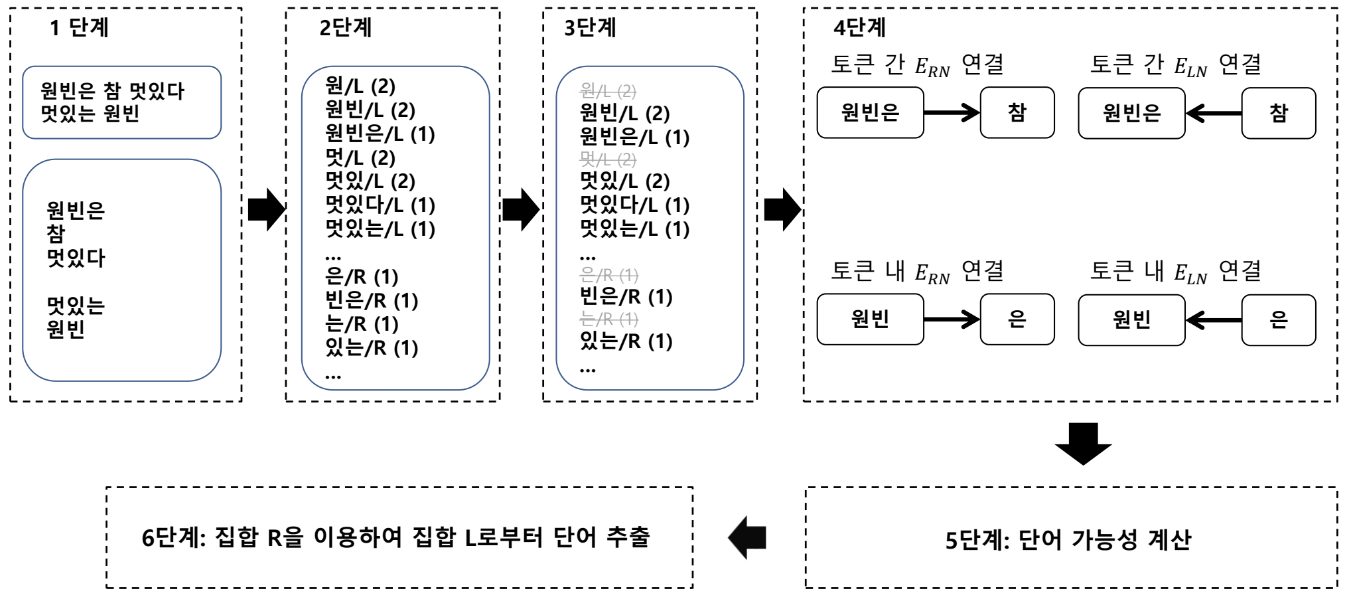
\includegraphics[keepaspectratio=true, width=0.9\linewidth]{figures/krwordrank_framework.png}
\caption{KR-WordRank 의 프레임워크}
\label{fig:korean_structure}
\end{figure}

여섯째, 필터링 과정을 거쳐 L + R 형태의 키워드를 제거한다. 부분어절 R 중 랭킹이 높은 순으로 $r_k$ 개의 부분어절을 선택한다. 이는 이 도메인에서 이용되는 조사 혹은 어미 집합이다. 키워드는 부분어절 L 에서만 선택한다. 부분어절 L 중 랭킹이 높은 순으로 정렬한 뒤, 랭킹이 낮은 $l$ 이 이미 선택된 키워듸 $w$ 와$[r_1, \dots r_{r_k}]$ 의 조합이 아니면 키워드 집합에 추가한다 (그림 \ref{tab:krwordrank_filtering}). 위의 예시에서 '원빈'이 키워드로 선택되면 '원빈 + [이, 은, 이다]' 는 키워드로 선택되지 않는다.

\begin{table}[H]
\centering
\label{tab:krwordrank_filtering}
\begin{tabular}{|l|}
\hline
\begin{tabular}[c]{@{}l@{}}W = \{\} \# keyword set\\ R = \{$r_1, r_2, \dots r_{r_k}$\} \# R set\\ L = {[}$l_1, l_2, \dots, l_l${]} \# L set sorted by rank\\ for l in L:\\ \quad if exist (w + R) in W:\\ \quad\quad pass\\ \quad else:\\ \quad\quad W  $\leftarrow$ W + \{l\}\end{tabular} \\ \hline
\end{tabular}
\caption{KR-WordRank 키워드 필터링 규칙}
\end{table}

%%%%%%%%%%%%%%%%%%%%%%%%%%%%%%%%%%%%%%%%%%%%%%%%%
\subsubsection{Performance}

제안된 KR-WordRank 의 성능을 확인하기 위하여 두 가지 실험을 수행하였다.
첫째는 단어의 정답이 기록되어 있는 세종 말뭉치를 이용하여 추출된 단어들이 실제로 단어인지 확인하였다.
키워드는 해석이 가능한 독립적인 단어이어야 하기 때문에 체언과 용언의 표현형, 관형사, 부사, 감탄사, 한 어절 이상을 이루는 복합형태소를 정답 단어 집합으로 이용하였다.
다섯 가지 단어 추출 기법에 대하여 추출된 단어의 정확도를 평가하였다.
WordRank 와 1음절을 제외한 Filtered WordRank, 그리고 $r_k$ 를 각각 300, 400, 500 으로 설정한 KR-WordRank 이다 (그림 \ref{fig:krwordrank_performance}).
WordRank 및 Filtered WordRank 는 상위에 랭크된 단어 후보들의 80\% 가까이 단어가 아니지만, KR-WordRank 를 이용하여 추출된 단어는 약 70\% 의 정확도를 보인다.

\begin{figure}[H]
\centering
\label{fig:krwordrank_performance}
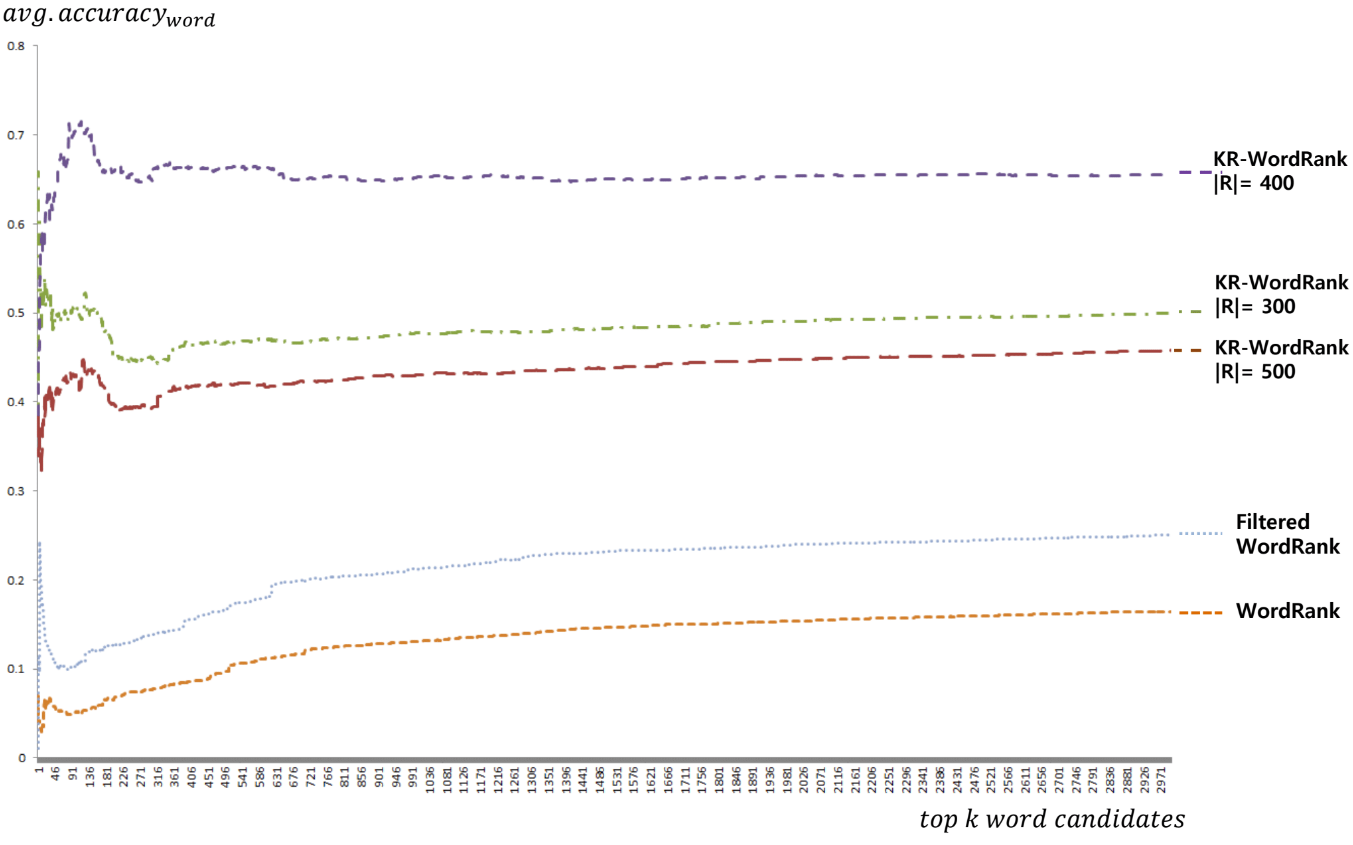
\includegraphics[keepaspectratio=true, width=0.9\linewidth]{figures/krwordrank_performance.png}
\caption{WordRank 와 KR-WordRank 를 이용하여 세종 말뭉치로부터 추출한 단어의 정확도}
\end{figure}

하지만 세종 말뭉치는 여러 주제의 문서들이 모여있는 말뭉치이며, 그래프 랭킹 기반 키워드 추출기는 단일한 주제의 문서 집합에서 잘 작동한다.
이 점을 확인하기 위하여 WordRank 와 KR-WordRank 를 이용하여 영화 "아저씨"의 영화평에서 키워드를 추출하였다 (그림 \ref{fig:krwordrank_vs_wordrank}).
문제 종류 A 는 해석이 불가능하거나 단어가 아닌 경우, B 는 조사나 어미가 결합된 어절, C 는 조사나 어미가 단어로 추출된 경우, D 는 복합명사인 경우이다.
문서 집합의 주제가 단일하더라도 WordRank 는 해석이 불가능한 1 음절을 키워드로 선택하는 경우가 많으며, 이는 대부분 조사나 어미로 추정된다.
WordRank 가 추출한 2 음절 이상의 키워드에는 '원빈의'와 같이 키워드와 조사가 결합된 경우와 2 음절 이상의 조사나 어미가 키워드로 추출된 경우가 많았다.
하지만 KR-WordRank 는 영화 '아저씨'를 대표하는 키워드들이 잘 추출되었으며, '한국영화'처럼 영화 도메인에서 자주 이용되는 복합명사도 키워드로 추출됨을 확인할 수 있다.

\begin{figure}[H]
\centering
\label{fig:krwordrank_vs_wordrank}
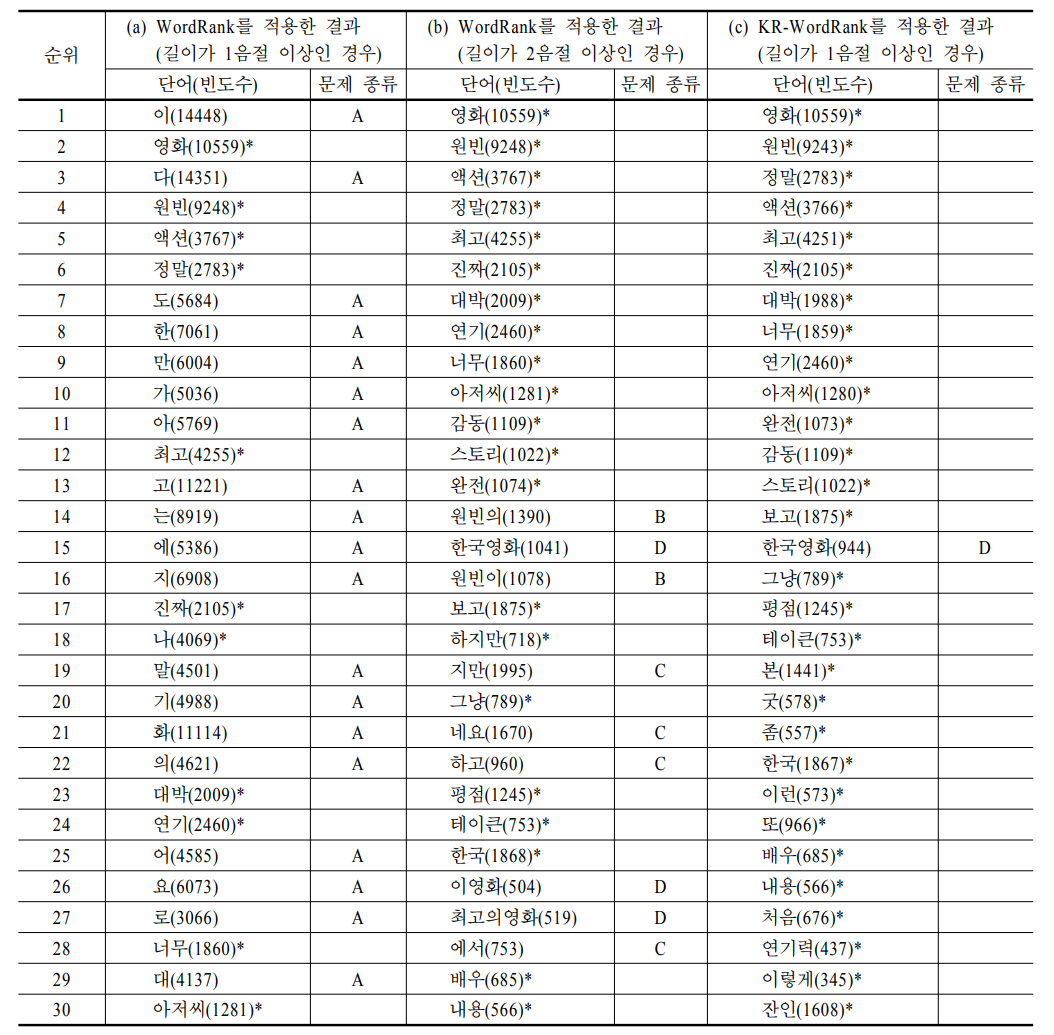
\includegraphics[keepaspectratio=true, width=0.9\linewidth]{figures/krwordrank_vs_wordrank.png}
\caption{WordRank 와 KR-WordRank 를 이용하여 추출한 영화 "아저씨" 리뷰의 키워드}
\end{figure}

%%%%%%%%%%%%%%%%%%%%%%%%%%%%%%%%%%%%%%%%%%%%%%%%%
\subsubsection{Conclusion}

제안된 알고리즘은 단어 사전과 같은 정보를 이용하지 않았음에도 불구하고 세종 말뭉치 기준 70\% 에 가까운 단어 추출 정확도를 보여주었다.
하지만 세종 말뭉치는 단일한 주제에 대한 문서 집합이 아니기 때문에 그래프 랭킹 기반 알고리즘을 이용하기에 적합하지 않다.
예시로 이용한 영화 "아저씨"의 영화평 텍스트는 단일한 주제의 텍스트이며, KR-WordRank 에 의하여 추출된 상위 랭크의 키워드들은 해당 문서 집합을 대표하는 단어이자 키워드임을 정성적으로 확인할 수 있다.


%%%%%%%%%%%%%%%%%%%%%%%%%%%%%%%%%%%%%%%%%%%%%%%%%%%%%%%%%%%%%%%%%%%%%%%%%%%%%%%
\subsection{Clustering and classification based method for heterogeneous texts}

%%%%%%%%%%%%%%%%%%%%%%%%%%%%%%%%%%%%%%%%%%%%%%%%%
\subsubsection{Document clustering}

앞 장에서 언급한 그래프 랭킹 기반 키워드 추출 방법은 문서 집합의 주제가 단일할 때 좋은 성능을 보이며, 여러 종류의 주제가 섞여있을 때에는 정보력이 적은 흔한 단어가 키워드로 선택된다.
이러한 점을 해결하기 위하여 LDA \citep{blei2003latent} 와 같은 토픽 모델링 및 토픽 레이블링 기법 \citep{sievert2014ldavis} 이 이용될 수 있다.
그러나 샘플링 기법을 기반으로 학습하는 LDA 는 문서 집합의 크기가 클 경우 많은 계산량이 필요하며 \citep{yuan2015lightlda}, 불용어제거와 같은 전처리 과정이 잘 이뤄지지 않으면 학습이 제대로 되지 않거나 불필요한 토픽과 단어들이 주요한 토픽과 단어로 해석되기도 한다 \citep{darling2011theoretical, newman2010evaluating}.
또한 LDA 는 하나의 문서에 여러 개의 주제가 존재한다는 가정을 한다.
하지만 뉴스나 블로그와 같이 길지 않은 문서는 사실 하나의 주제를 가지는 경우가 많으며, 이떄는 문서 군집화 역시 토픽 모델링으로 이용할 수 있다 \citep{dhillon2001concept, xu2003document}.

군집화 알고리즘은 Gaussian Mixture Model (GMM), Density-based model (ester1996density), Hierarchical clustering \citep{zhao2005hierarchical} 등의 방법이 존재하지만, 고차원 벡터로 표현되는 문서의 특징과 계산 비용을 고려하면 k-means \citep{lloyd1982least} 는 매우 유용한 문서 군집화 알고리즘이다.

군집화 알고리즘의 목적은 하나의 데이터셋을 여러 개의 부분 집합으로 분리하는 것으로, 각 부분 집합의 데이터 간에는 유사도가 높고 각 부분 집합 간에는 유사도가 낮은 부분 집합을 탐색하는 것이다.
부분 집합, 군집의 개수가 $k$ 개로 정해질 경우, 이 문제를 k-partition 문제라 명한다.
하지만 식 \ref{eq:kpartition} 은 NP-hard 문제이기 때문에 최적의 값을 찾기 어렵다.

\begin{equation}
\centering
\label{eq:kpartition}
\sum _{i=1}^{k}\sum _{\mathbf {x} \in S_{i}}\left\|\mathbf {x} -{\boldsymbol {\mu }}_{i}\right\|^{2}
\end{equation}

이를 효율적으로 근사하기 위하여 k-means \citep{lloyd1982least} 가 제안되었으며, 빠른 계산 속도와 적은 메모리 사용, 분산 계산이 쉬운 구조적 특징 때문에 대량의 데이터 군집화에 널리 이용되고 있다.
k-means 는 그림 \ref{fig:lloyd_kmeans} 의 과정으로 학습된다.
초기 군집 대표값 (initial centroids) 를 선정한 뒤, 데이터의 모든 점을 가장 가까운 군집 대표값의 레이블로 할당한다.
각 군집에 속한 데이터의 평균을 새로운 군집 대표값으로 설정한 뒤, 위 과정을 모델이 수렴할 때까지 반복한다.

\begin{figure}[H]
\centering
\begin{tabular}{|l|}
\hline
\begin{tabular}[c]{@{}l@{}}
$D$: dataset\\
$k$: a number of clusters\\
\\
\textbf{def kmeans} ($D, k$):\\
\quad $C$ $\leftarrow$ Initialize $k$ centroids with random sampling\\
\quad $L$ $\leftarrow$- Assign all points to its closest centroid\\
\quad while (not converged):\\
\quad \quad $C$ $\leftarrow$ Update centroids by averaging assigned date points \\
\quad \quad $L$ $\leftarrow$ Reassign all the points to its closest centroid\\
\quad \textbf{return} $C$, $L$

\end{tabular} \\ \hline
\end{tabular}
\caption{Lloyd k-means}
\label{fig:lloyd_kmeans}
\end{figure}

문서 군집화에는 문서 간 거리 척도의 설정이 중요하다.
일반적으로 문서는 bag-of-words model 과 같은 고차원 스파스 벡터나 Doc2Vec 과 같은 고차원의 분산 표상 표현 (distributed representation) 으로 표현된다 \citep{le2014distributed, dai2015document}.
Bag-of-words model 로 표현되는 문서 간의 유사도는 두 문서에 공통으로 등장한 단어 정보가 중요하지만, 유컬리디언 거리 는 이를 제대로 표현하지 못하기 때문에 코싸인 거리 혹은 자카드 거리와 같은 척도를 이용해야 한다 \citep{huang2008similarity}.
문서가 분산 표상 표현으로 표현된다 하더라도 임베딩 공간에서 두 객체의 유사도는 코싸인 거리를 이용하는 것이 좋다 \citep{levy2015improving}.

유컬리디언 거리 대신 코싸인 거리를 이용하는 k-means 를 spherical k-means \citep{dhillon2001concept} 라 하며, 이는 문서 군집화에 적합한 방법이다.

%%%%%%%%%%%%%%%%%%%%%%%%%%%%%%%%%%%%%%%%%%%%%%%%%
\subsubsection{Improved initializer of k-means for document clustering}

k-means 는 초기 군집 대표값 (initial points) 에 의하여 군집화의 결과가 바뀔 수 있으며, 널리 퍼진 점들을 초기 군집 대표값으로 선택해야 안정적인 학습이 가능하다.
kmeans++ \citep{arthur2007k} 은 이를 위하여 제안된 방법으로, 다음의 과정을 반복하여 초기 군집 대표값을 선택한다 (그림 \ref{fig:kmeanspp}).
처음 한 점 $c_0$ 는 임의로 선택한 뒤 이 점을 기준으로 다른 모든 점들과의 거리를 계산하여 그 제곱에 비례한 확률로 다른 점을 선택하여 널리 퍼진 점들을 초기 군집 대표값으로 선택한다.

\begin{figure}[H]
\centering
\begin{tabular}{|l|}
\hline
\begin{tabular}[c]{@{}l@{}}

1. Select point $c_1$ randomly \\
2. Select next point $c_t$ with probability $\frac{d(c_{t-1}, c_t)^2}{\sum d(c_{t-1}, c_t)^2}$ \\
3. Repeat step 2 until $k$ points are chosen as initial points.\\

\end{tabular} \\ \hline
\end{tabular}
\caption{k-means++}
\label{fig:kmeanspp}
\end{figure}

하지만 bag-of-words model 이나 문서 임베딩 공간이 이용하는 고차원 공간에서는 대부분의 거리값이 일정해지는 성질이 있으며, 사실상 가까운 점들과 먼 점들로 이분할 되는 현상이 발생한다 \citep{aggarwal2001surprising}.
그렇기 때문에 k-means++ 의 두 번째 단계에서 학습되는 확률 분포는 uniform 분포에 가깝게 되어 많은 계산 비용만 발생한다.
또한 이전에 선택된 초기 군집 대표값을 기준으로 멀리 떨어진 점을 선택하기 때문에 $c_{t-2}$ 와 $c_t$ 가 멀리 떨어진 점이라는 보장을 하기 어렵다.

이를 해결하기 위하여 문서 군집화에 적합한 효율적인 k-means 초기화 방법을 제안한다 (그림 \ref{fig:proposed_initializer}).

첫째, 데이터에서 $\alpha \times k$ 개의 점을 임의로 선택하여 $D_{init}$ 을 만든다.
거의 대부분의 데이터 간 거리가 동일하여 초기값을 선택하기 위하여 모든 점을 고려할 필요가 없기 때문이다.

둘째, $D_{init}$ 에서 임의의 한 점 $c_i$ 을 선택한다.

셋째, $D_{init}$ 에서 $c_i$ 와 거리가 $t_{init}$ 보다 작은 모든 점을 제거한다.
이를 통하여 $t_{init}$ 보다 가까운 두 점이 초기 군집 대표값으로 선택되는 것을 방지할 수 있다.

넷째, $k$ 개의 점이 선택될 때 까지 2 - 3 과정을 반복한다.

다섯째, 2 - 3 과정에서 $k$ 개의 점을 선택하지 못하면 $D - D_{init}$ 에서 나머지 점을 임의로 선택한다.

\begin{figure}[H]
\centering
%\resizebox{\textwidth}{!}
{\begin{tabular}{|l|}
\hline
\begin{tabular}[c]{@{}l@{}}
\small

1. Construct set $D_{init}$, $\alpha \times k$ randomly selected data from data $D$\\
2. Select $c_i$ randomly from $D_{init}$\\
3. Remove $x_j$ where $x_j \in D_{init}$ and cos($⁡c_{i}, x_{j}$) $\ge t_{init}$\\
4. Repeat 2 – 3 until $k$ centroid points are selected or $D_{init}$ becomes empty\\
5. If the number of selected centroid is less than $k$, then select\\ 
\quad remaining points from $D - D_{init}$ randomly\\

\end{tabular} \\ \hline
\end{tabular}}
\caption{Proposed initialization method}
\label{fig:proposed_initializer}
\end{figure}

이 과정은 데이터의 일부의 점만을 초기값 설정에 이용하기 때문에 계산이 빠르며, 3 번 과정으로 인하여 서로 멀리 떨어진 점들을 초기값으로 설정할 수 있다.
이는 고차원 문서 벡터 공간의 대부분의 거리가 같다는 특징을 이용한 것이다.


%%%%%%%%%%%%%%%%%%%%%%%%%%%%%%%%%%%%%%%%%%%%%%%%%
\subsubsection{Document clustering labeling}

각 군집별로 키워드를 추출함으로써 군집 레이블링을 할 수 있다.
키워드는 한 군집에서 자주 등장하며, 다른 군집과 구분할 수 있는 단어여야 한다 \citep{snyder2013topic}.
군집 레이블을 문서들의 레이블로 이용하여 문서 분류기를 학습함으로써 키워드를 추출할 수도 있지만 \citep{zhang2006keyword, onan2016ensemble}, 이는 문서 분류기를 추가르 학습해야만 한다.
반면 토픽 레이블링을 위해 제안된 방법들은 토픽 벡터의 값으로부터 간단한 통계를 통하여 키워드를 추출한다 \citep{chuang2012termite, snyder2013topic}.
이 장에서는 추가적인 모델의 학습을 하지 않는 문서 레이블링을 위한 키워드 추출 방법을 제안한다.

k-means 는 학습 결과로 각 문서가 속한 군집의 레이블과 군집 별 대표 벡터 (centroid vectors) 를 얻을 수 있다.
문서가 분산 표상 표현의 벡터로 입력되더라도 군집 레이블을 이용하여 bag-of-words model 형태의 군집 별 대표 벡터를 만들 수 있다.
Bag-of-words model 형태의 군집 대표 벡터를 L1 정규화하면 군집 내 문서에서의 단어 분포 확률 벡터로 해석할 수 있다.
식 \ref{eq:proposed_labeler} 은 각 군집 $c_i$ 에서 단어 $w$ 의 키워드 점수로, $p_i(w)$ 는 군집 $c_i$ 에서의 단어 $w$ 가 등장한 확률이며, $p_{-i}(w)$ 는 군집 $i$ 를 제외한 문서 집합에서의 단어 $w$ 의 등장 확률 분포이다.

\begin{equation}
\label{eq:proposed_labeler}
\centering
s(w, c_i) = \frac{p_i (w)}{p_i (w) + p_{-i}(w)}
\end{equation}

이 값이 클수록 distinctiveness 를 지니는데, 단어 $w$ 가 군집 $c_i$ 에서만 등장할 경우 1 을, 다른 문서 집합과 동일한 분포로 등장할 경우 0.5 의 값을 가진다.
하지만 희귀한 단어는 1 에 가까운 값을 지니는 경우가 많다.
이를 방지 하기 위하여 각 군집별로 $p_i(w)$ 가 큰 $k_0$ 개의 단어를 선택한 뒤 식 \ref{eq:proposed_labeler} 가 큰 $k_1$ 개의 단어를 선택하면 saliency 와 distinctiveness 를 모두 지닌 키워드를 선택할 수 있다.
이 과정은 추가적인 모델의 학습이 필요하지 않기 때문에 군집의 개수가 많더라도 빠르게 군집 별 키워드를 추출할 수 있다.

%%%%%%%%%%%%%%%%%%%%%%%%%%%%%%%%%%%%%%%%%%%%%%%%%
\subsubsection{Merging similar cluster}

k-means 의 단점 중 하나는 각 군집의 크기가 서로 다를 경우, 이들이 같은 크기의 군집으로 학습되는 uniform effect 현상이 발생한다 \citep{xiong2009k}.
이를 해결하기 위해서는 하나의 군집을 작은 여러 개의 군집들로 표현해야 하기 때문에 군집의 개수는 예상하는 군집 개수보다 크게 설정하는 것이 좋다 \citep{liang2012k}.
큰 크기의 클래스가 여러 개로 나뉘어질 경우 후처리로 병합이 가능하지만, 크기가 작은 클래스가 여러 개의 큰 군집으로 나뉘어질 경우 이들의 복원은 매우 어렵기 때문이다.

하지만 군집의 개수가 많으면 하나의 주제에 대한 문서 집합이 여러 개의 군집으로 나뉘어진다.
이를 해결하기 위하여 그림 \ref{fig:kmeans_postprocessing} 의 후처리 과정을 거칠 수 있다.
먼저 군집의 문서 개수 역순으로 각 군집을 정렬한 뒤, 첫번째 군집을 병합된 하나의 군집 $M_j$ 로 할당한다.
두번째 큰 군집부터 순차적으로 모든 병합된 군집과 유사도를 계산한다.
만약 병합된 군집 $M_j$ 에 속한 모든 군집들과 $t_merge$ 이상의 유사도를 지니면 이를 $M_j$ 에 추가하고, 그렇지 않으면 독립적인 새로운 병합된 군집을 만든다.
이 과정을 이용하면 크기가 작은 클래스도 독립적인 군집으로 추출하면서 큰 클래스가 여러 개의 중복된 군집으로 나뉘어지는 것을 방지할 수 있다.

\begin{figure}[H]
\centering
% \resizebox{\textwidth}{!}
{\begin{tabular}{|l|}
\hline
\begin{tabular}[c]{@{}l@{}}

1. Sort clusters $C_1, C_2, \dots, C_k$ by their document frequency in decreasing order.\\
2. For centroid $c_i$,\\
\quad if there exists a merged cluster $M_j$, in which $\forall c_p \in M_j, cos{(c_i, c_p)} \ge t_{merge}$,\\
\quad \quad $M_j \leftarrow M_j \cup \{ C_i \}$\\
\quad else\\
\quad \quad create new merged cluster $M_j$ = $\{C_i\}$\\

\end{tabular} \\ \hline
\end{tabular}}
\caption{Merging similar clusters with similarity threshold}
\label{fig:kmeans_postprocessing}
\end{figure}

%%%%%%%%%%%%%%%%%%%%%%%%%%%%%%%%%%%%%%%%%%%%%%%%%
\subsubsection{Subword tokenizer to solve out of vocabulary}




%%%%%%%%%%%%%%%%%%%%%%%%%%%%%%%%%%%%%%%%%%%%%%%%%
\subsubsection{Franework of proposed method}

그림 \ref{fig:pseudocode} 은 제안하는 문서 군집화 알고리즘의 의사 코드이다.
제안하는 방법은 대량의 문서 군집화를 위한 빠른 초기화 알고리즘과 중복된 군집을 병합하기 위한 후처리 기능, 그리고 군집 대표 벡터를 이용한 군집 레이블링 기능이 포함되어 있다.
사용자는 $\alpha$ 와 $t_{init}$ 를 통하여 초기화에 이용할 점들의 개수와 초기화된 점들 간의 거리를 조절할 수 있으며, $t_{merge}$ 를 통하여 병합된 군집의 크기를 조절할 수 있다.
또한 $k_0$ 와 $k_1$ 을 이용하여 군집 별 키워드 및 후보 단어의 개수를 조절할 수 있다.

\begin{figure}[H]
\centering
\begin{tabular}{|l|}
\hline
\begin{tabular}[c]{@{}l@{}}
$D$: dataset\\
$k$: a number of clusters\\
$t_{init}$: minimum distance for initializer\\
$t_{merge}$: threshold for merging similar clusters\\
$k_0$: number of keyword candidates\\
$k_1$: number of selected keywords\\
\\
\textbf{def improved\_kmeans} ($D, k, \alpha, t_{init}, t_{merge}, k_0, k_1$):\\
\quad $C$ $\leftarrow$ Initialize $k$ centroids with sparse initializer ($D, k, \alpha, t_{init}$)\\
\quad $L$ $\leftarrow$- Assign all points to its closest centroid\\
\quad while (not converged):\\
\quad \quad $C$ $\leftarrow$ Update centroid. Averaging their belonging points \\
\quad \quad $L$ $\leftarrow$ Reassign all the points to its closest centroid\\
\quad $C$ $\leftarrow$ merge similar cluster ($C, L, t_{merge}$)\\
\quad $Z$ $\leftarrow$ cluster labeling ($C, L, k_0, k_1$)\\
\quad \textbf{return} $C$, $L$, $Z$

\end{tabular} \\ \hline
\end{tabular}
\caption{Pseudo code of improved k-means}
\label{fig:pseudocode}
\end{figure}


%%%%%%%%%%%%%%%%%%%%%%%%%%%%%%%%%%%%%%%%%%%%%%%%%
\subsubsection{Performance}


\begin{table}[H]
\centering
\caption{Example of cluster labels from k=1,000 clustering result with IMDb reviews}
\label{tab:imdb_cluster_label}
\resizebox{\textwidth}{!}{\begin{tabularx}{\textwidth}{sb}
\hline

Cluster category & Cluster labels \\ \hline
"Titanic" & iceberg, zane, sinking, titanic, rose, winslet, camerons, 1997, leonardo, leo, ship, cameron, dicaprio, kate, tragedy, jack, disaster, james, romance, love, effects, story\\ \hline
Heros of Marvel comics & zemo, chadwick, boseman, bucky, panther, holland, cap, infinity, mcu, russo, civil, bvs, antman, winter, ultron, airport, avengers, marvel, captain, superheroes, stark, evans, america, iron, spiderman\\ \hline
Alien sci-fi & skyline, jarrod, balfour, strause, invasion, independence, cloverfield, angeles, district, los, worlds, aliens, alien, la, budget, scifi, battle, cgi, day, effects, war\\ \hline
Horror & gayheart, loretta, candyman, legends, urban, witt, campus, tara, reid, legend, alicia, englund, leto, scream, murders, slasher, helen, killer, student, teen, summer, cut, horror, final, sequel, scary \\ \hline
"Matrix" & neo, morpheus, neos, oracle, trinity, zion, architect, hacker, reloaded, revolutions, wachowski, fishburne, machines, agents, matrix, keanu, smith, reeves, agent, jesus, machine, computer, fighting, fight, real \\ \hline

\end{tabularx}}
\end{table}


%%%%%%%%%%%%%%%%%%%%%%%%%%%%%%%%%%%%%%%%%%%%%%%%%
\subsubsection{Conclusion}


%%%%%%%%%%%%%%%%%%%%%%%%%%%%%%%%%%%%%%%%%%%%%%%%%%%%%%%%%%%%%%%%%%%%%%%%%%%%%%%
\section{Topic detection using unsupervised sequence segmentation}



%%%%%%%%%%%%%%%%%%%%%%%%%%%%%%%%%%%%%%%%%%%%%%%%%%%%%%%%%%%%%%%%%%%%%%%%%%%%%%%
\bibliography{reference}

\end{document}
